\documentclass[aspectratio=169]{beamer}

% ---------- Theme & Colours ----------
\usetheme{Madrid}
\usecolortheme{default}

%% ── Rashidul's colour palette ──
\definecolor{NavyBlue}{RGB}{31,56,137}
\definecolor{LightBlue}{RGB}{173,198,230}
\definecolor{DarkBlue}{RGB}{20,40,100}
\definecolor{AlertRed}{RGB}{180,30,30}
\definecolor{GreenOK}{RGB}{30,140,60}
\definecolor{CarRed}{RGB}{220,50,50}
\definecolor{CarOrange}{RGB}{230,130,30}
\definecolor{CarGreen}{RGB}{50,160,50}
\definecolor{CarBlue}{RGB}{65, 105, 225}
\definecolor{CarGray}{RGB}{150,150,150}
\definecolor{SkinTone}{RGB}{240,195,160}
\definecolor{HairDark}{RGB}{40,30,20}
\definecolor{HairBlue}{RGB}{25,50,110}
\definecolor{ShirtRed}{RGB}{190,40,40}
\definecolor{ShirtTeal}{RGB}{30,120,130}
\definecolor{CloudGreen}{RGB}{50,170,80}
\definecolor{BubbleYellow}{RGB}{240,200,30}

%% ── Mobin/Riyad's colour palette ──
\definecolor{maincolor}{RGB}{0,102,204}
\definecolor{accentcolor}{RGB}{255,102,0}
\definecolor{lightgray}{RGB}{240,240,240}
\definecolor{successcolor}{RGB}{46,125,50}

%% ── Default beamer colours (Rashidul style – used for Part 1) ──
\setbeamercolor{palette primary}{bg=NavyBlue,fg=white}
\setbeamercolor{palette secondary}{bg=DarkBlue,fg=white}
\setbeamercolor{palette tertiary}{bg=NavyBlue,fg=white}
\setbeamercolor{palette quaternary}{bg=DarkBlue,fg=white}
\setbeamercolor{structure}{fg=NavyBlue}
\setbeamercolor{section in toc}{fg=NavyBlue}
\setbeamercolor{block title}{bg=NavyBlue,fg=white}
\setbeamercolor{block body}{bg=LightBlue!25,fg=black}
\setbeamercolor{alerted text}{fg=AlertRed}
\setbeamercolor{frametitle}{bg=NavyBlue,fg=white}
\setbeamercolor{title}{fg=white,bg=NavyBlue}
\setbeamerfont{frametitle}{size=\large,series=\bfseries}

% ---------- Packages ----------
\usepackage{tikz}
\usetikzlibrary{arrows.meta, shapes.geometric, shapes.callouts, positioning, decorations.pathreplacing, calc, backgrounds, fit, shapes, arrows}
\usepackage{amsmath, amssymb}
\usepackage{booktabs}
\usepackage{xcolor}
\usepackage{ifthen}
\usepackage{algorithm}
\usepackage{algorithmic}
\usepackage{graphicx}

% ---------- Footer ----------
\setbeamertemplate{footline}{%
  \leavevmode%
  \hbox{%
    \begin{beamercolorbox}[wd=.333\paperwidth,ht=2.25ex,dp=1ex,center]{palette secondary}%
      \usebeamerfont{author in head/foot}\insertshortauthor
    \end{beamercolorbox}%
    \begin{beamercolorbox}[wd=.334\paperwidth,ht=2.25ex,dp=1ex,center]{palette primary}%
      \usebeamerfont{title in head/foot}\insertshorttitle
    \end{beamercolorbox}%
    \begin{beamercolorbox}[wd=.333\paperwidth,ht=2.25ex,dp=1ex,right]{palette secondary}%
      \usebeamerfont{date in head/foot}\insertshortdate{}\hspace*{2em}
      \insertframenumber{} / \inserttotalframenumber\hspace*{2ex}
    \end{beamercolorbox}}%
  \vskip0pt%
}
\setbeamertemplate{navigation symbols}{}

%% Macro: cartoon face (from Rashidul)
\newcommand{\cartoonface}[5]{%
  \begin{scope}[shift={(#1,#2)}, scale=#3]
    \fill[SkinTone] (-0.10,-0.44) rectangle (0.10,-0.20);
    \fill[#5] (-0.55,-1.05) -- (-0.30,-0.44) -- (0.30,-0.44) -- (0.55,-1.05) -- cycle;
    \fill[SkinTone, draw=HairDark, line width=0.5pt] (0,0) circle (0.42cm);
    \ifthenelse{\equal{#4}{w}}{%
      \fill[HairDark]
        (-0.42,0.05) .. controls (-0.48,0.45) and (-0.20,0.72) .. (0,0.72)
        .. controls (0.20,0.72) and (0.48,0.45) .. (0.42,0.05)
        .. controls (0.46,-0.10) and (0.52,-0.25) .. (0.50,-0.38)
        -- (0.38,-0.30)
        .. controls (0.38,0.00) and (0.44,0.05) .. (0.42,0.05)
        -- cycle;
      \fill[HairDark]
        (-0.42,0.05) .. controls (-0.44,0.05) and (-0.38,0.00) .. (-0.38,-0.30)
        -- (-0.50,-0.38)
        .. controls (-0.52,-0.25) and (-0.46,-0.10) .. (-0.42,0.05);
    }{%
      \fill[HairDark]
        (-0.42,0.08) .. controls (-0.44,0.40) and (-0.18,0.68) .. (0,0.68)
        .. controls (0.18,0.68) and (0.44,0.40) .. (0.42,0.08) -- cycle;
    }
    \fill[white] (-0.16,0.05) ellipse (0.10cm and 0.07cm);
    \fill[white] ( 0.16,0.05) ellipse (0.10cm and 0.07cm);
    \fill[HairDark] (-0.14,0.05) circle (0.045cm);
    \fill[HairDark] ( 0.18,0.05) circle (0.045cm);
    \draw[HairDark, line width=0.6pt] (-0.26,0.17) .. controls (-0.18,0.21) .. (-0.06,0.17);
    \draw[HairDark, line width=0.6pt] ( 0.06,0.17) .. controls ( 0.18,0.21) .. ( 0.26,0.17);
    \fill[SkinTone!60!HairDark] (0,-0.06) circle (0.03cm);
    \draw[HairDark, line width=0.7pt]
      (-0.14,-0.18) .. controls (-0.07,-0.26) and (0.07,-0.26) .. (0.14,-0.18);
    \fill[SkinTone, draw=HairDark, line width=0.4pt]
      (-0.44,-0.03) ellipse (0.07cm and 0.10cm);
    \fill[SkinTone, draw=HairDark, line width=0.4pt]
      ( 0.44,-0.03) ellipse (0.07cm and 0.10cm);
  \end{scope}
}

% ---------- Title Info ----------
\title[MOEA/D]{Multi-Objective Evolutionary Algorithms based on Decomposition (MOEA/D)}
\author[Rashidul, Mobin, Riyad]{Md.\ Rashidul Islam \and Fathum Mobin \and Md.\ Riyadun Nabi \\ 2205072 \qquad \qquad 2205073 \qquad \qquad 2205076}
\date[February 2026]{23 February 2026}

% ============================================================
\begin{document}
% ============================================================

%% ---- Title Slide ----
\begin{frame}
  \titlepage
\end{frame}

%% ============================================================
%% PART 1: MOTIVATION & BACKGROUND (Speaker 1 — Md. Rashidul Islam)
%% ============================================================
% ============================================================

%% ---- Title Slide ----


% %% ============================================================
% %% HOOK SLIDE — Insert immediately AFTER \titlepage frame
% %%              and BEFORE the "What Will You Learn Today?" frame
% %% ============================================================

% \begin{frame}[plain]
% \begin{center}

% % ---------------- STEP 1 ----------------
% \onslide<1->{
% \vspace{1.8em}
% {\large\color{NavyBlue!60} Today We will talk about}\\[0.8em]

% {\fontsize{32}{36}\selectfont\bfseries\color{NavyBlue}
% MOEA/D}\\[0.5em]

% {\normalsize\color{DarkBlue}
% \textbf{M}ulti-\textbf{O}bjective
% \textbf{E}volutionary
% \textbf{A}lgorithm
% by
% \textbf{D}ecomposition}
% }

% \vspace{1.2em}

% % ---------------- STEP 2 ----------------
% \onslide<2->{
% \begin{tikzpicture}
% \node[draw=NavyBlue!30, fill=NavyBlue!6, rounded corners=8pt,
%       font=\normalsize, inner sep=14pt, text width=8.5cm, text centered]
%   {A powerful \textbf{evolutionary algorithm}\\
%    for solving \textbf{multi-objective optimization} problems.};
% \end{tikzpicture}
% }

% \vspace{1.6em}

% % ---------------- STEP 3 — PIVOT ----------------
% \onslide<3->{
% {\large\color{NavyBlue!70}
% But before we understand the algorithm...}
% }

% \vspace{0.8em}

% \onslide<4->{
% \begin{tikzpicture}
% \node[draw=NavyBlue, fill=NavyBlue!10, rounded corners=10pt,
%       font=\large\bfseries, inner sep=18pt, text width=8.0cm,
%       text centered, text=NavyBlue]
%   {we must understand the \emph{problem}.};
% \end{tikzpicture}
% }

% \end{center}
% \end{frame}

%% ============================================================
%% HOOK SLIDE 1 — Big acronym reveal on dark background
%% ============================================================
{
\setbeamertemplate{footline}{}
\setbeamercolor{palette primary}{bg=DarkBlue,fg=DarkBlue}
\setbeamercolor{palette secondary}{bg=DarkBlue,fg=DarkBlue}
\setbeamercolor{palette tertiary}{bg=DarkBlue,fg=DarkBlue}
\setbeamercolor{palette quaternary}{bg=DarkBlue,fg=DarkBlue}
\setbeamertemplate{background}{%
  
\begin{tikzpicture}
    \useasboundingbox (0,0) rectangle (\paperwidth,\paperheight);
    \fill[DarkBlue] (0,-1cm) rectangle (\paperwidth,\paperheight);
    \fill[NavyBlue] (0,\paperheight-0.55cm) rectangle (\paperwidth,\paperheight);
  \end{tikzpicture}%
}
\begin{frame}[plain]

\begin{center}
\vspace{0.6em}
{\color{LightBlue!70}\footnotesize\bfseries\MakeUppercase{Today we will talk about}}

\vspace{1.0em}

{\fontsize{72}{76}\selectfont\bfseries\color{white}
MOEA/D}

\vspace{0.5em}

\onslide<1->{
{\color{LightBlue!80}\normalsize
\textbf{\color{white}M}ulti-\textbf{\color{white}O}bjective\ %
\textbf{\color{white}E}volutionary\ %
\textbf{\color{white}A}lgorithm based on \textbf{\color{white}D}ecomposition}
}

\vspace{1.4em}

\onslide<2->{
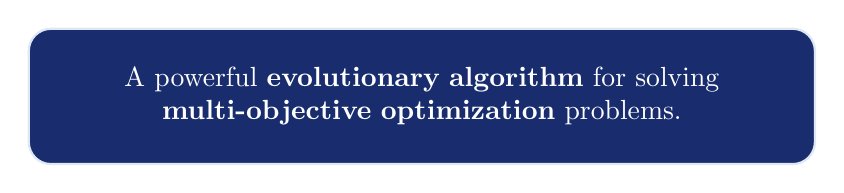
\begin{tikzpicture}
\node[draw=LightBlue!40, fill=NavyBlue!80!black, rounded corners=8pt,
      font=\normalsize\color{white}, inner sep=14pt, text width=9.0cm,
      text centered, line width=0.8pt]
  {A powerful \textbf{evolutionary algorithm} for solving\\
   \textbf{multi-objective optimization} problems.};
\end{tikzpicture}
}
\end{center}
\end{frame}
}

%% ============================================================
%% HOOK SLIDE 2 — Dramatic pivot: "But first… the PROBLEM"
%% ============================================================
{
\setbeamertemplate{footline}{}
\setbeamercolor{palette primary}{bg=DarkBlue,fg=DarkBlue}
\setbeamercolor{palette secondary}{bg=DarkBlue,fg=DarkBlue}
\setbeamercolor{palette tertiary}{bg=DarkBlue,fg=DarkBlue}
\setbeamercolor{palette quaternary}{bg=DarkBlue,fg=DarkBlue}
\setbeamertemplate{background}{%
  
\begin{tikzpicture}
    \useasboundingbox (0,0) rectangle (\paperwidth,\paperheight);
    \fill[DarkBlue] (0,-1cm) rectangle (\paperwidth,\paperheight);
  \end{tikzpicture}%
}
\begin{frame}[plain]

\begin{center}
\vspace{2.2em}

\onslide<1->{
{\large\color{white!70}
But before we understand the algorithm\ldots}
}

\vspace{2.0em}

\onslide<2->{

\begin{tikzpicture}
\node[
  draw=LightBlue, fill=NavyBlue, rounded corners=12pt,
  line width=2.2pt, inner sep=22pt, text width=13cm, text centered
]{
  {\fontsize{26}{32}\selectfont\bfseries\color{white}
  we must understand\\[0.3em]
  \textcolor{LightBlue!90}{what \emph{multi-objective optimization} is.}}
};
\end{tikzpicture}
}

\end{center}
\end{frame}
}

%% =========================================================
%% SLIDE 2 — ML Model Provocation (animated)
%% =========================================================
\begin{frame}{What Is the Best Machine Learning Model?}

\begin{center}
{\small\itshape
Three models trained on the same dataset. Same task. Different trade-offs.}
\end{center}

\vspace{0.9cm}

\begin{columns}[c]

% =====================================================
% MODEL A
% =====================================================
\column{0.33\textwidth}
\centering
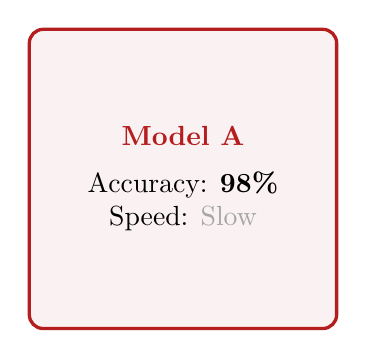
\begin{tikzpicture}
\node[
  draw=AlertRed,
  fill=AlertRed!6,
  rounded corners=5pt,
  line width=1.2pt,
  minimum width=3.6cm,
  minimum height=3.8cm,
  inner sep=10pt
]{
\begin{minipage}{3.2cm}
\centering
{\bfseries\color{AlertRed} Model A}

\vspace{0.5em}

Accuracy: {\bfseries 98\%}

Speed: {\color{gray!70} Slow}
\end{minipage}
};
\end{tikzpicture}

% =====================================================
% MODEL B
% =====================================================
\column{0.33\textwidth}
\centering
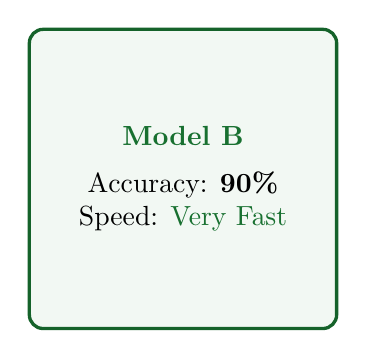
\begin{tikzpicture}
\node[
  draw=GreenOK!70!black,
  fill=GreenOK!6,
  rounded corners=5pt,
  line width=1.2pt,
  minimum width=3.6cm,
  minimum height=3.8cm,
  inner sep=10pt
]{
\begin{minipage}{3.2cm}
\centering
{\bfseries\color{GreenOK!80!black} Model B}

\vspace{0.5em}

Accuracy: {\bfseries 90\%}

Speed: {\color{GreenOK!80!black} Very Fast}
\end{minipage}
};
\end{tikzpicture}

% =====================================================
% MODEL C
% =====================================================
\column{0.33\textwidth}
\centering
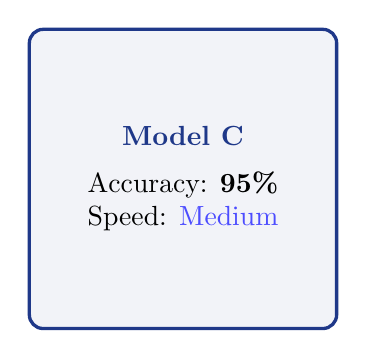
\begin{tikzpicture}
\node[
  draw=NavyBlue,
  fill=NavyBlue!6,
  rounded corners=5pt,
  line width=1.2pt,
  minimum width=3.6cm,
  minimum height=3.8cm,
  inner sep=10pt
]{
\begin{minipage}{3.2cm}
\centering
{\bfseries\color{NavyBlue} Model C}

\vspace{0.5em}

Accuracy: {\bfseries 95\%}

Speed: {\color{blue!70} Medium}
\end{minipage}
};
\end{tikzpicture}

\end{columns}

\vspace{0.8cm}

% =====================================================
% FINAL QUESTION
% =====================================================
\only<2>{
\begin{center}

\begin{tikzpicture}
\node[
  draw=AlertRed,
  fill=AlertRed!5,
  rounded corners=4pt,
  line width=1.2pt,
  inner sep=8pt,
  minimum width=8cm
]{
{\large\bfseries\color{AlertRed}
Which model is optimal?}
};
\end{tikzpicture}
\end{center}
}

\end{frame}

%% =========================================================
%% SLIDE 3 — The Realization (animated)
%% =========================================================
% \begin{frame}[plain]
%   \begin{tikzpicture}[remember picture, overlay]
%     %% Light background wash
%     \fill[NavyBlue!6]
%       (current page.south west) rectangle (current page.north east);
%     %% Top accent bar
%     \fill[NavyBlue]
%       (current page.north west) rectangle
%       ([yshift=-0.45cm]current page.north east);
%     %% Bottom accent bar
%     \fill[NavyBlue]
%       (current page.south west) rectangle
%       ([yshift=0.45cm]current page.south east);
%   \end{tikzpicture}

%   \vspace{1.5em}

%   \begin{center}

%     %% BIG STATEMENT
%     \only<1->{%
%       \begin{tikzpicture}
%         \node[
%           draw=NavyBlue, fill=white,
%           rounded corners=7pt, line width=2pt,
%           inner sep=14pt, minimum width=13cm
%         ] {%
%           \fontsize{22}{28}\selectfont\bfseries\color{NavyBlue}
%           There is no single best model.%
%         };
%       \end{tikzpicture}
%     }

%     \vspace{1.0em}

%     %% REFRAME
%     \only<2->{%
%       \begin{tikzpicture}
%         \node[
%           draw=DarkBlue!40, fill=NavyBlue!10,
%           rounded corners=5pt, line width=1pt,
%           inner sep=10pt, minimum width=11cm
%         ] {%
%           \fontsize{14}{18}\selectfont\color{DarkBlue}
%           It depends on \textbf{what you value.}%
%         };
%       \end{tikzpicture}
%     }

%     \vspace{0.9em}

    % %% INSIGHT LINE
    % \only<3->{%
    %   \begin{tikzpicture}
    %     %% Two opposing labels
    %     \node[
    %       fill=AlertRed, text=white,
    %       rounded corners=4pt, font=\bfseries\normalsize,
    %       inner sep=6pt, minimum width=3.6cm
    %     ] (acc) at (-3.5,0) {Accuracy};

    %     \node[
    %       fill=GreenOK, text=white,
    %       rounded corners=4pt, font=\bfseries\normalsize,
    %       inner sep=6pt, minimum width=3.6cm
    %     ] (spd) at (3.5,0) {Speed};

    %     %% Arrow with label
    %     \draw[-{Stealth[length=7pt]}, AlertRed!70, line width=2pt]
    %       (acc.east) -- ++(1.3,0);
    %     \draw[-{Stealth[length=7pt]}, GreenOK!70, line width=2pt]
    %       (spd.west) -- ++(-1.3,0);

    %     \node[
    %       font=\bfseries\small, text=gray!70!black,
    %       fill=white, draw=gray!40, rounded corners=3pt,
    %       inner sep=4pt
    %     ] at (0,0) {vs};

    %     %% Caption below
    %     \node[
    %       font=\itshape\small, text=gray!60!black,
    %       align=center
    %     ] at (0,-0.75) {Trade-offs are unavoidable.};
    %   \end{tikzpicture}
    % }

%   \end{center}
% \end{frame}

%% =========================================================
%% SLIDE — General Real-World Motivation
%% =========================================================
\begin{frame}{Why Does This Matter? Real-World Trade-Offs}

  \begin{center}
    {\small\itshape Most decisions in the real world force you to balance competing priorities.}
  \end{center}

  \vspace{0.6em}

  \begin{columns}[c]
    \column{0.55\textwidth}

    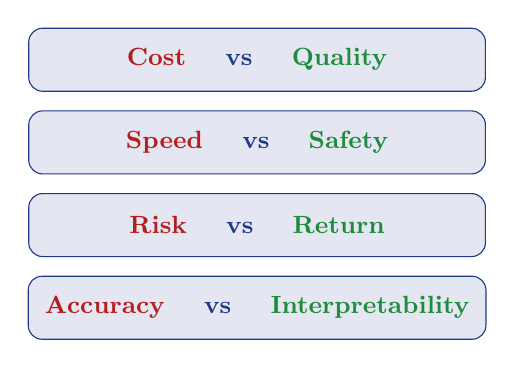
\begin{tikzpicture}[
      bullet/.style={draw=NavyBlue, fill=NavyBlue!12, rounded corners=5pt,
                     minimum width=5.8cm, minimum height=0.80cm,
                     align=center, font=\small\bfseries, text=NavyBlue,
                     inner sep=6pt}
    ]
      \node[bullet] (b1) at (0, 0)    {\textcolor{AlertRed}{Cost} \quad vs \quad \textcolor{GreenOK}{Quality}};
      \node[bullet] (b2) at (0,-1.05) {\textcolor{AlertRed}{Speed} \quad vs \quad \textcolor{GreenOK}{Safety}};
      \node[bullet] (b3) at (0,-2.10) {\textcolor{AlertRed}{Risk} \quad vs \quad \textcolor{GreenOK}{Return}};
      \node[bullet] (b4) at (0,-3.15) {\textcolor{AlertRed}{Accuracy} \quad vs \quad \textcolor{GreenOK}{Interpretability}};
    \end{tikzpicture}

    \column{0.42\textwidth}
    \onslide<2->{
      \begin{block}{}
        \centering
        \textbf{Most real-world problems involve conflicting objectives.}\\[0.4em]
        {\small Improving one goal often means compromising another.}
      \end{block}
    }
  \end{columns}

\end{frame}


%% ---- Two Persons Animated Slide ----

%% Colour palette for cartoon faces
\definecolor{SkinTone}{RGB}{240,195,160}
\definecolor{HairDark}{RGB}{40,30,20}
\definecolor{HairBlue}{RGB}{25,50,110}
\definecolor{ShirtRed}{RGB}{190,40,40}
\definecolor{ShirtTeal}{RGB}{30,120,130}
\definecolor{CloudGreen}{RGB}{50,170,80}
\definecolor{BubbleYellow}{RGB}{240,200,30}

%% Macro: cartoon face
%% Args: cx, cy, scale, hair-style (w=woman / m=man), shirt-color
\newcommand{\cartoonface}[5]{%
  \begin{scope}[shift={(#1,#2)}, scale=#3]
    %% Neck
    \fill[SkinTone] (-0.10,-0.44) rectangle (0.10,-0.20);
    %% Shirt body
    \fill[#5] (-0.55,-1.05) -- (-0.30,-0.44) -- (0.30,-0.44) -- (0.55,-1.05) -- cycle;
    %% Face circle
    \fill[SkinTone, draw=HairDark, line width=0.5pt] (0,0) circle (0.42cm);
    %% Hair
    \ifthenelse{\equal{#4}{w}}{%
      %% Woman: dark bob covering top+sides
      \fill[HairDark]
        (-0.42,0.05) .. controls (-0.48,0.45) and (-0.20,0.72) .. (0,0.72)
        .. controls (0.20,0.72) and (0.48,0.45) .. (0.42,0.05)
        .. controls (0.46,-0.10) and (0.52,-0.25) .. (0.50,-0.38)
        -- (0.38,-0.30)
        .. controls (0.38,0.00) and (0.44,0.05) .. (0.42,0.05)
        -- cycle;
      \fill[HairDark]
        (-0.42,0.05) .. controls (-0.44,0.05) and (-0.38,0.00) .. (-0.38,-0.30)
        -- (-0.50,-0.38)
        .. controls (-0.52,-0.25) and (-0.46,-0.10) .. (-0.42,0.05);
    }{%
      %% Man: short neat hair on top only
      \fill[HairDark]
        (-0.42,0.08) .. controls (-0.44,0.40) and (-0.18,0.68) .. (0,0.68)
        .. controls (0.18,0.68) and (0.44,0.40) .. (0.42,0.08) -- cycle;
    }
    %% Eyes (white + pupil)
    \fill[white] (-0.16,0.05) ellipse (0.10cm and 0.07cm);
    \fill[white] ( 0.16,0.05) ellipse (0.10cm and 0.07cm);
    \fill[HairDark] (-0.14,0.05) circle (0.045cm);
    \fill[HairDark] ( 0.18,0.05) circle (0.045cm);
    %% Eyebrows (slightly furrowed = determined look)
    \draw[HairDark, line width=0.6pt] (-0.26,0.17) .. controls (-0.18,0.21) .. (-0.06,0.17);
    \draw[HairDark, line width=0.6pt] ( 0.06,0.17) .. controls ( 0.18,0.21) .. ( 0.26,0.17);
    %% Nose dot
    \fill[SkinTone!60!HairDark] (0,-0.06) circle (0.03cm);
    %% Mouth (slight smile)
    \draw[HairDark, line width=0.7pt]
      (-0.14,-0.18) .. controls (-0.07,-0.26) and (0.07,-0.26) .. (0.14,-0.18);
    %% Ear marks
    \fill[SkinTone, draw=HairDark, line width=0.4pt]
      (-0.44,-0.03) ellipse (0.07cm and 0.10cm);
    \fill[SkinTone, draw=HairDark, line width=0.4pt]
      ( 0.44,-0.03) ellipse (0.07cm and 0.10cm);
  \end{scope}
}

\begin{frame}{Real-World Example: Buying a Car}

\begin{center}
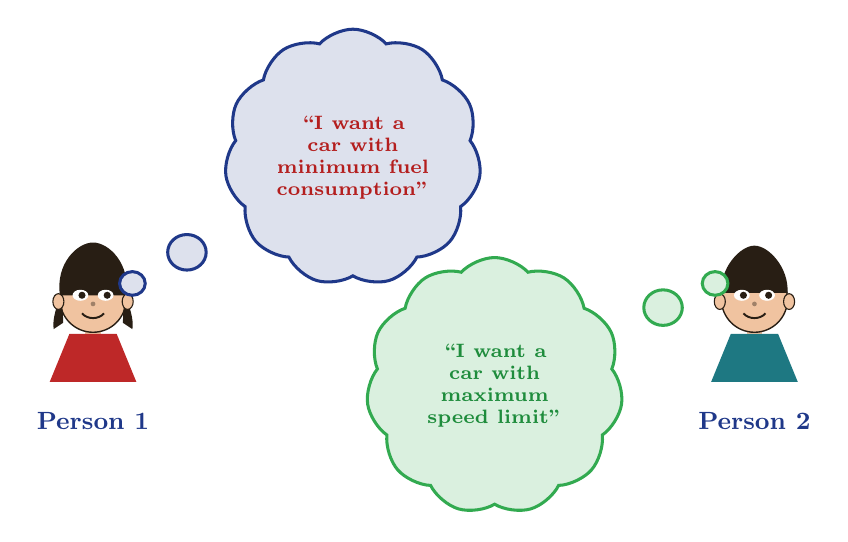
\begin{tikzpicture}

%% =========================================================
%% PERSON 1  (left, woman)
%% =========================================================
\onslide<1->{

  % Cartoon face
  \cartoonface{-4.2}{0.0}{1.0}{w}{ShirtRed}

  % Name label
  \node[font=\small\bfseries, text=NavyBlue]
    at (-4.2,-1.55) {Person 1};

  % Cloud callout (top right, pointing left)
  \node[
    cloud callout,
    cloud puffs=11,
    cloud puff arc=95,
    minimum width=2.0cm,
    minimum height=1.4cm,
    draw=NavyBlue,
    fill=NavyBlue!15,
    callout absolute pointer={(-3.7,0.2)},
    text width=2.0cm,
    align=center,
    font=\scriptsize\bfseries,
    inner sep=1.8pt,
    line width=1.1pt
  ] at (-0.9,1.8)
  {
    \textcolor{AlertRed}
    {``I want a car with minimum fuel consumption''}
  };
}

%% =========================================================
%% PERSON 2  (right, man)
%% =========================================================
\onslide<2->{

  % Cartoon face
  \cartoonface{4.2}{0.0}{1.0}{m}{ShirtTeal}

  % Name label
  \node[font=\small\bfseries, text=NavyBlue]
    at (4.2,-1.55) {Person 2};

  % Cloud callout (bottom left, pointing right)
  \node[
    cloud callout,
    cloud puffs=11,
    cloud puff arc=95,
    minimum width=2.0cm,
    minimum height=1.4cm,
    draw=CloudGreen,
    fill=CloudGreen!18,
    callout absolute pointer={(3.7,0.2)},
    text width=2.0cm,
    align=center,
    font=\scriptsize\bfseries,
    inner sep=1.8pt,
    line width=1.1pt
  ] at (0.9,-1.1)
  {
    \textcolor{GreenOK}
    {``I want a car with maximum speed limit''}
  };
}

\end{tikzpicture}
\end{center}

\onslide<3->{
\begin{center}
  \alert{\textbf{Both objectives matter --- but they conflict with each other!}}
\end{center}
}

\end{frame}

\begin{frame}{A Real-World Example: Buying a Car}

\begin{center}
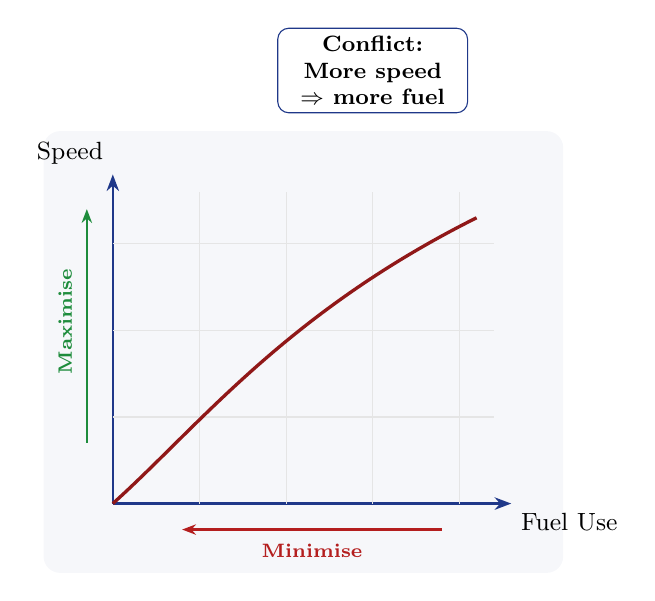
\begin{tikzpicture}[scale=1.1]

  % Soft background panel
  \fill[NavyBlue!4, rounded corners=6pt]
        (-0.8,-0.8) rectangle (5.2,4.3);

  % Axes
  \draw[-{Stealth[length=6pt]}, thick, NavyBlue]
        (0,0) -- (4.6,0);

  \draw[-{Stealth[length=6pt]}, thick, NavyBlue]
        (0,0) -- (0,3.8);

  % Axis labels
  \node[below right, font=\small]
        at (4.6,0) {Fuel Use};

  \node[above left, font=\small]
        at (0,3.8) {Speed};

  % Light grid
  \draw[gray!20, thin]
        (1,0)--(1,3.6)
        (2,0)--(2,3.6)
        (3,0)--(3,3.6)
        (4,0)--(4,3.6);

  \draw[gray!20, thin]
        (0,1)--(4.4,1)
        (0,2)--(4.4,2)
        (0,3)--(4.4,3);

  % RANDOM TRADE-OFF CURVE (smooth Bezier)
  \draw[very thick, AlertRed!80!black]
        (0,0)
        .. controls (1.0,0.9)
        and (2.0,2.2)
        .. (4.2,3.3);

  % OUTSIDE minimise (x-axis direction)
  \node[AlertRed, font=\scriptsize\bfseries]
        at (2.3,-0.55) {Minimise};

  \draw[AlertRed, thick, -{Stealth[length=5pt]}]
        (3.8,-0.30) -- (0.8,-0.30);

  % OUTSIDE maximise (y-axis direction)
  \node[GreenOK, font=\scriptsize\bfseries, rotate=90]
        at (-0.55,2.1) {Maximise};

  \draw[GreenOK, thick, -{Stealth[length=5pt]}]
        (-0.30,0.7) -- (-0.30,3.4);

  % Transparent conflict annotation box
  \node[
    draw=NavyBlue,
    fill=none,
    rounded corners=4pt,
    font=\footnotesize\bfseries,
    align=center,
    inner sep=3pt,
    text width=2.2cm
  ]
  at (3.0,5.0)
  {Conflict:\\ More speed $\Rightarrow$ more fuel};

\end{tikzpicture}
\end{center}

\end{frame}
\begin{frame}{Four Cars on the Shortlist}
  They agree on four candidate cars. Can we shrink the list?

  \vspace{0.4em}
  \begin{columns}[c]
    \column{0.52\textwidth}
    \begin{center}
    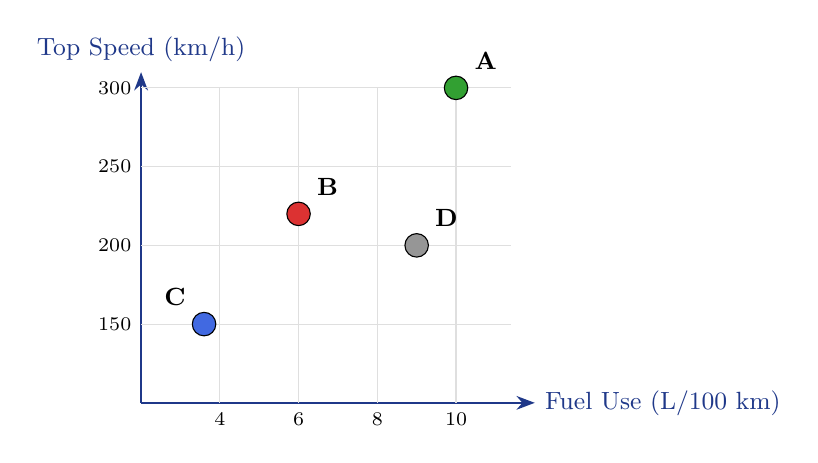
\begin{tikzpicture}[scale=1.0]
      % axes
      \draw[-{Stealth}, thick, NavyBlue] (0,0) -- (5.0,0)
            node[right, font=\small] {Fuel Use (L/100 km)};
      \draw[-{Stealth}, thick, NavyBlue] (0,0) -- (0,4.2)
            node[above, font=\small] {Top Speed (km/h)};

      % grid
      \foreach \x in {1,2,3,4}
        \draw[gray!25,thin] (\x,0)--(\x,4.0);
      \foreach \y in {1,2,3,4}
        \draw[gray!25,thin] (0,\y)--(4.7,\y);

      % axis labels
      \foreach \x/\lbl in {1/4, 2/6, 3/8, 4/10}
        \node[font=\scriptsize, below] at (\x,0) {\lbl};
      \foreach \y/\lbl in {1/150, 2/200, 3/250, 4/300}
        \node[font=\scriptsize, left] at (0,\y) {\lbl};

      % Car A
      \onslide<1->{
        \node[circle, fill=CarGreen, draw=black, inner sep=3pt,
              label={[font=\small\bfseries]above right:A}]
              at (4.0, 4.0) {};
      }

      % Car B
      \onslide<2->{
        \node[circle, fill=CarRed, draw=black, inner sep=3pt,
              label={[font=\small\bfseries]above right:B}]
              at (2.0, 2.4) {};
      }

      % Car C
      \onslide<3->{
        \node[circle, fill=CarBlue, draw=black, inner sep=3pt,
              label={[font=\small\bfseries]above left:C}]
              at (0.8, 1.0) {};
      }

      % Car D
      \onslide<4->{
        \node[circle, fill=CarGray, draw=black, inner sep=3pt,
              label={[font=\small\bfseries]above right:D}]
              at (3.5, 2.0) {};
      }

    \end{tikzpicture}
    \end{center}

    \column{0.45\textwidth}
    \small
    \begin{tabular}{ccc}
      \toprule
      \textbf{Car} & \textbf{Speed} & \textbf{Fuel} \\
      \midrule

      \onslide<1->{\textcolor{CarGreen}{\textbf{A}}} & \onslide<1->{300 km/h} & \onslide<1->{10 L/100} \\

      \onslide<2->{\textcolor{CarRed}{\textbf{B}}}   & \onslide<2->{220 km/h} & \onslide<2->{ 6 L/100} \\

      \onslide<3->{\textcolor{CarBlue}{\textbf{C}}} & \onslide<3->{150 km/h} & \onslide<3->{ 4 L/100} \\

      \onslide<4->{\textcolor{CarGray}{\textbf{D}}}  & \onslide<4->{200 km/h} & \onslide<4->{ 9 L/100} \\

      \bottomrule
    \end{tabular}

    \vspace{0.8em}
    \onslide<5->{
      \textbf{Goal:} Maximise speed,\\
      \phantom{\textbf{Goal:}} Minimise fuel use.

      \vspace{0.4em}
      \alert{Can we remove any car?}
    }

  \end{columns}
\end{frame}

% %% ============================================================
% %% SECTION 2
% %% ============================================================
\begin{frame}[plain]
  \begin{center}
    \vspace{3em}
    {\Huge\bfseries\color{NavyBlue} Dominance \& Non-Domination}
  \end{center}
\end{frame}

%% =========================================================
%% DOMINANCE — Merged Slide: Intuition + Formal Conditions
%% =========================================================
\begin{frame}{The Key Concept: Dominance}

\begin{center}

\onslide<1->{
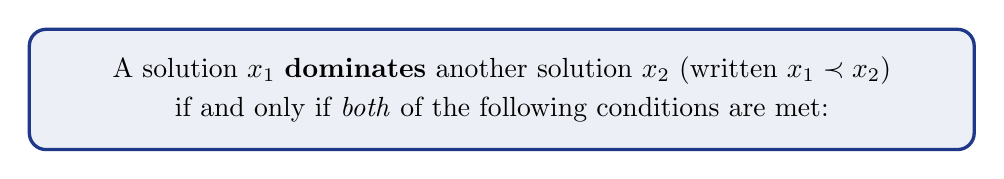
\begin{tikzpicture}
  \node[draw=NavyBlue, fill=NavyBlue!8, rounded corners=6pt,
        line width=1.2pt, inner sep=10pt, minimum width=12cm, align=center]
  {%
    A solution $x_1$ \textbf{dominates} another solution $x_2$
    (written $x_1 \prec x_2$)\\[0.2em]
    if and only if \emph{both} of the following conditions are met:
  };
\end{tikzpicture}
}

\vspace{0.8em}

\onslide<2->{

\begin{tikzpicture}
  \node[draw=NavyBlue, fill=NavyBlue!10, rounded corners=5pt,
        line width=1pt, inner sep=10pt, minimum width=12cm, align=left, font=\normalsize]
  {%
    \textbf{\textcolor{NavyBlue}{Condition\ 1 --- No Worse in All Objectives:}}\\[0.3em]
    $x_1$ is \textbf{no worse} than $x_2$ in \emph{every} objective.
  };
\end{tikzpicture}
}

\vspace{0.6em}

\onslide<3->{
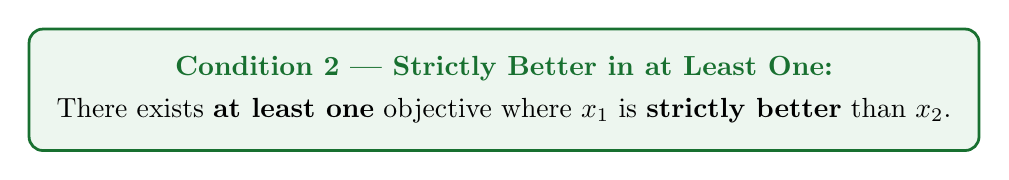
\begin{tikzpicture}
  \node[draw=GreenOK!80!black, fill=GreenOK!8, rounded corners=5pt,
        line width=1pt, inner sep=10pt, minimum width=12cm, align=center, font=\normalsize]
  {%
    \textbf{\textcolor{GreenOK!80!black}{Condition\ 2 --- Strictly Better in at Least One:}}\\[0.3em]
    There exists \textbf{at least one} objective where $x_1$ is \textbf{strictly better} than $x_2$.
  };
\end{tikzpicture}
}

\end{center}

\end{frame}


%% =========================================================
%% DOMINANCE — Slide D: Visual — All Cars on Plot (animated)
%% =========================================================
\begin{frame}{Visualising Dominance: All Four Cars}

  \begin{columns}[c]
    \column{0.55\textwidth}
    \begin{center}
    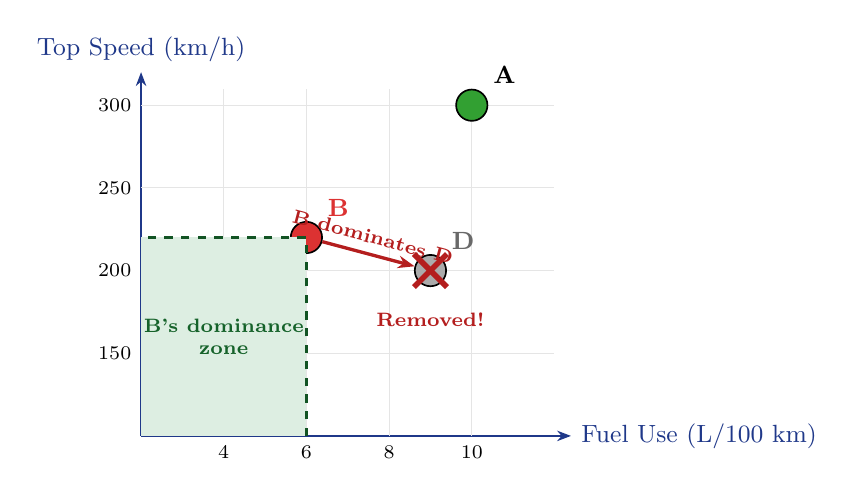
\begin{tikzpicture}[scale=1.05]
      % Axes
      \draw[-{Stealth[length=5pt]}, NavyBlue, thick]
        (0,0) -- (5.2,0) node[right, font=\small] {Fuel Use (L/100 km)};
      \draw[-{Stealth[length=5pt]}, NavyBlue, thick]
        (0,0) -- (0,4.4) node[above, font=\small] {Top Speed (km/h)};
      % Grid
      \foreach \x in {1,2,3,4}
        \draw[gray!20,thin] (\x,0)--(\x,4.2);
      \foreach \y in {1,2,3,4}
        \draw[gray!20,thin] (0,\y)--(5.0,\y);
      % Tick labels
      \foreach \x/\lbl in {1/4, 2/6, 3/8, 4/10}
        \node[font=\scriptsize, below] at (\x,0) {\lbl};
      \foreach \y/\lbl in {1/150, 2/200, 3/250, 4/300}
        \node[font=\scriptsize, left] at (0,\y) {\lbl};

      % Step 1: Show all four cars
      \onslide<1->{
        \node[circle, fill=CarGreen, draw=black, line width=0.6pt, inner sep=4pt,
              label={[font=\small\bfseries]above right:A}] (A) at (4.0,4.0) {};
        \node[circle, fill=CarRed, draw=black, line width=0.6pt, inner sep=4pt,
              label={[font=\small\bfseries, text=CarRed]above right:B}] (B) at (2.0,2.4) {};
        \node[circle, fill=CarGreen, draw=black, line width=0.6pt, inner sep=4pt,
              label={[font=\small\bfseries]above left:C}] (C) at (0.8,1.0) {};
        \node[circle, fill=CarGray!80, draw=black, line width=0.6pt, inner sep=4pt,
              label={[font=\small\bfseries, text=CarGray!70!black]above right:D}] (D) at (3.5,2.0) {};
      }

      % Step 2: Highlight B's dominance zone
      \onslide<2->{
        \fill[GreenOK!15] (0,0) rectangle (2.0,2.4);
        \draw[dashed, GreenOK!60!black, thick]
          (2.0,0) -- (2.0,2.4) -- (0,2.4);
        \node[font=\scriptsize\bfseries, text=GreenOK!70!black, align=center]
          at (1.0,1.2) {B's dominance\\zone};
      }

      % Step 3: Arrow from B to D
      \onslide<3->{
        \draw[-{Stealth[length=6pt]}, AlertRed, very thick]
          (B) -- (D) node[midway, above,  font=\scriptsize\bfseries, text=AlertRed, sloped]
          {B dominates D};
      }

      % Step 4: Cross out D
      \onslide<4->{
        \draw[AlertRed, very thick, line width=2pt] (3.3,1.8) -- (3.7,2.2);
        \draw[AlertRed, very thick, line width=2pt] (3.7,1.8) -- (3.3,2.2);
        \node[font=\scriptsize\bfseries, text=AlertRed] at (3.5,1.4) {Removed!};
      }

    \end{tikzpicture}
    \end{center}

    \column{0.42\textwidth}

    \onslide<1->{
      \textbf{Our four candidates:}\\[0.3em]
      \small
      \begin{tabular}{lcc}
        \toprule
        \textbf{Car} & \textbf{Speed} & \textbf{Fuel} \\
        \midrule
        A & 300 km/h & 10 L \\
        B & 220 km/h & 6 L \\
        C & 150 km/h & 4 L \\
        D & 200 km/h & 9 L \\
        \bottomrule
      \end{tabular}
    }

    \vspace{0.6em}

    \onslide<2->{
      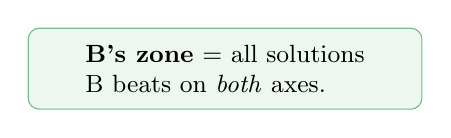
\begin{tikzpicture}
        \node[draw=GreenOK!60, fill=GreenOK!8, rounded corners=4pt,
              inner sep=6pt, minimum width=5.0cm, align=left, font=\small] {%
          \textbf{B's zone} = all solutions\\
          B beats on \emph{both} axes.
        };
      \end{tikzpicture}
    }

    \vspace{0.4em}

    \onslide<3->{
      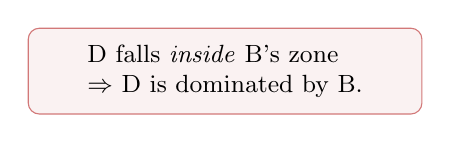
\begin{tikzpicture}
        \node[draw=AlertRed!60, fill=AlertRed!6, rounded corners=4pt,
              inner sep=6pt, minimum width=5.0cm, align=left, font=\small] {%
          D falls \emph{inside} B's zone\\
          $\Rightarrow$ D is dominated by B.
        };
      \end{tikzpicture}
    }

    \vspace{0.4em}

    \onslide<4->{
      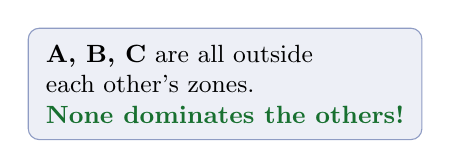
\begin{tikzpicture}
        \node[draw=NavyBlue!50, fill=NavyBlue!8, rounded corners=4pt,
              inner sep=6pt, minimum width=5.0cm, align=left, font=\small] {%
          \textbf{A, B, C} are all outside\\
          each other's zones.\\
          \textcolor{GreenOK!80!black}{\bfseries None dominates the others!}
        };
      \end{tikzpicture}
    }

  \end{columns}
\end{frame}

%% =========================================================
%% MERGED — Pairwise Comparisons + Pareto Front
%% =========================================================
\begin{frame}{The Remaining Cars Form the Pareto Front}

\begin{columns}[c]

% ================= LEFT: Compact pairwise summary =================
\column{0.48\textwidth}

\onslide<1->{
\begin{center}
{\small\itshape Can A, B, or C dominate each other?}
\end{center}

\vspace{0.3em}

\small
\begin{tabular}{cccc}
  \toprule
  \textbf{Pair} & \textbf{Speed} & \textbf{Fuel} & \textbf{Result} \\
  \midrule
  A vs B & A \textcolor{GreenOK}{\checkmark} & B \textcolor{GreenOK}{\checkmark} & \textbf{No dominance} \\
  A vs C & A \textcolor{GreenOK}{\checkmark} & C \textcolor{GreenOK}{\checkmark} & \textbf{No dominance} \\
  B vs C & B \textcolor{GreenOK}{\checkmark} & C \textcolor{GreenOK}{\checkmark} & \textbf{No dominance} \\
  \bottomrule
\end{tabular}
}

\vspace{0.5em}

\onslide<2->{
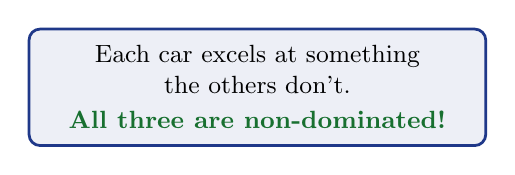
\begin{tikzpicture}
  \node[draw=NavyBlue, fill=NavyBlue!8, rounded corners=4pt,
        line width=1pt, inner sep=6pt, minimum width=5.8cm,
        align=center, font=\small]
  {%
    Each car excels at something\\
    the others don't.\\[0.2em]
    \textcolor{GreenOK!80!black}{\bfseries All three are non-dominated!}
  };
\end{tikzpicture}
}


% ================= RIGHT: Pareto front graph =================
\column{0.50\textwidth}

\onslide<2->{
\begin{center}
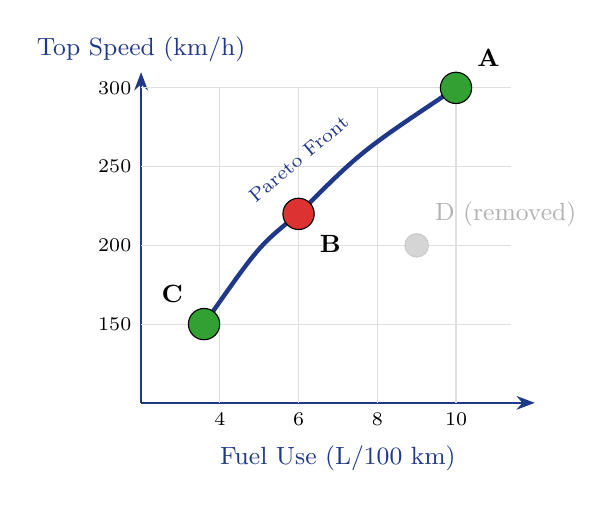
\begin{tikzpicture}[scale=1.0]
  \draw[-{Stealth}, thick, NavyBlue] (0,0) -- (5.0,0)
        node[font=\small] at (2.5,-0.7) {Fuel Use (L/100 km)};
  \draw[-{Stealth}, thick, NavyBlue] (0,0) -- (0,4.2)
        node[above, font=\small] {Top Speed (km/h)};
  \foreach \x in {1,2,3,4}
    \draw[gray!25,thin] (\x,0)--(\x,4.0);
  \foreach \y in {1,2,3,4}
    \draw[gray!25,thin] (0,\y)--(4.7,\y);
  \foreach \x/\lbl in {1/4, 2/6, 3/8, 4/10}
    \node[font=\scriptsize, below] at (\x,0) {\lbl};
  \foreach \y/\lbl in {1/150, 2/200, 3/250, 4/300}
    \node[font=\scriptsize, left] at (0,\y) {\lbl};
  % Non-dominated front curve
  \draw[NavyBlue, ultra thick] (0.8,1.0) .. controls (1.5,2.0) .. (2.0,2.4)
                                         .. controls (2.8,3.2) .. (4.0,4.0);
  \node[font=\scriptsize, text=NavyBlue, rotate=40] at (2,3.1)
        {Pareto Front};
  % Cars A, B, C (non-dominated)
  \node[circle, fill=CarGreen, draw=black, inner sep=4pt,
        label={[font=\small\bfseries]above right:A}] (A) at (4.0, 4.0) {};
  \node[circle, fill=CarRed,   draw=black, inner sep=4pt,
        label={[font=\small\bfseries]below right:B}] (B) at (2.0, 2.4) {};
  \node[circle, fill=CarGreen, draw=black, inner sep=4pt,
        label={[font=\small\bfseries]above left:C}]  (C) at (0.8, 1.0) {};
  % D faded
  \node[circle, fill=CarGray!40, draw=gray!40, inner sep=3pt,
        label={[font=\small, text=gray!60]above right:D (removed)}]
        (D) at (3.5, 2.0) {};
\end{tikzpicture}
\end{center}
}

\end{columns}
\end{frame}

\begin{frame}{The Goal of Multi-Objective Optimization}

% ------------------------------------------------
% Fundamental Goal (Top)
% ------------------------------------------------
\begin{block}{The Fundamental Goal}
Multi-objective optimization aims to 
\textbf{find (or approximate) the entire non-dominated set} — 
giving the decision-maker the full picture of trade-offs.
\end{block}

\vspace{0.6em}

% ------------------------------------------------
% Concept Diagram (Middle)
% ------------------------------------------------
\begin{center}

\begin{tikzpicture}[
  box/.style={
    draw=NavyBlue,
    fill=NavyBlue!12,
    rounded corners=6pt,
    minimum width=3.2cm,
    minimum height=1.1cm,
    align=center,
    font=\small\bfseries,
    text=NavyBlue
  },
  arrow/.style={-{Stealth[length=6pt]}, NavyBlue, thick}
]

\node[box] (A) at (0,0)
  {Multiple\\ Conflicting Objectives};

\node[box] (B) at (4.8,0)
  {Dominance\\ Concept};

\node[box] (C) at (9.6,0)
  {Non-Dominated\\ Set (Pareto Front)};

\draw[arrow] (A) -- (B)
  node[midway, above, font=\scriptsize]{defines};

\draw[arrow] (B) -- (C)
  node[midway, above, font=\scriptsize]{identifies};

\end{tikzpicture}
\end{center}

\vspace{0.8em}

% ------------------------------------------------
% Final Distilled Statement (Bottom)
% ------------------------------------------------
% \begin{center}
% \begin{tikzpicture}
% \node[
%   draw=GreenOK!80!black,
%   fill=GreenOK!12,
%   rounded corners=6pt,
%   line width=1.2pt,
%   inner sep=8pt,
%   text width=9.5cm,
%   text centered,
%   font=\small
% ]
% {
% \textbf{Discover all trade-off solutions that cannot be improved without sacrifice.}
% };
% \end{tikzpicture}
% \end{center}

\end{frame}


\begin{frame}{What if there are millions of solutions?}

  % STEP 1 — Show only the question
  \onslide<1->{
  \begin{block}{The Challenge}
    Imagine you have \textbf{millions of possible solutions} to a problem.
    You cannot try them all. How do you find a good one \emph{fast}?
  \end{block}
  }

  \vspace{0.1em}

  \begin{columns}[T]

    % STEP 2 — Random search appears
    \column{0.48\textwidth}
    \onslide<2->{
    \textbf{A bad strategy: Random Search}\\[0.4em]
    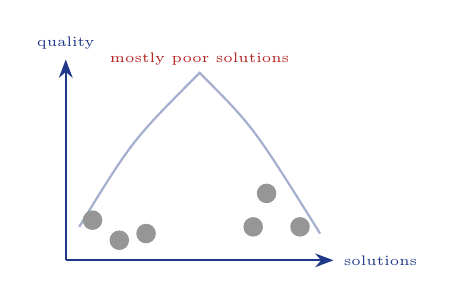
\begin{tikzpicture}[scale=0.85]
      \draw[-{Stealth}, NavyBlue, thick] (0,0)--(4,0)
            node[right, font=\tiny]{solutions};
      \draw[-{Stealth}, NavyBlue, thick] (0,0)--(0,3)
            node[above, font=\tiny]{quality};

      \draw[NavyBlue!40, thick]
            (0.2,0.5) .. controls (1,1.8) .. (2.0,2.8)
            .. controls (2.8,2.0) .. (3.8,0.4);

      \foreach \x/\y in {0.4/0.6, 1.2/0.4, 3.5/0.5, 0.8/0.3, 3.0/1.0, 2.8/0.5}
        \node[circle, fill=CarGray, inner sep=2.5pt] at (\x,\y) {};

      \node[font=\tiny, text=AlertRed] at (2.0, 3.0) {mostly poor solutions};
    \end{tikzpicture}

    {\small Picking random solutions wastes most attempts on bad regions.}
    }

    % STEP 3 — Guided improvement appears
    \column{0.48\textwidth}
    \onslide<3->{
    \textbf{A smarter strategy: Learn \& Improve}\\[0.4em]
    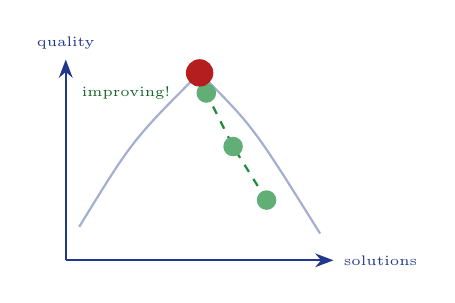
\begin{tikzpicture}[scale=0.85]
      \draw[-{Stealth}, NavyBlue, thick] (0,0)--(4,0)
            node[right, font=\tiny]{solutions};
      \draw[-{Stealth}, NavyBlue, thick] (0,0)--(0,3)
            node[above, font=\tiny]{quality};

      \draw[NavyBlue!40, thick]
            (0.2,0.5) .. controls (1,1.8) .. (2.0,2.8)
            .. controls (2.8,2.0) .. (3.8,0.4);

      \draw[-{Stealth}, GreenOK, thick, dashed]
            (3.0,0.9) -- (2.5,1.7) -- (2.1,2.5) -- (2.0,2.8);

      \foreach \x/\y in {3.0/0.9, 2.5/1.7, 2.1/2.5}
        \node[circle, fill=GreenOK!70, inner sep=2.5pt] at (\x,\y) {};

      \node[circle, fill=AlertRed, inner sep=3.5pt] at (2.0,2.8) {};
      \node[font=\tiny, text=GreenOK!70!black] at (0.9,2.5) {improving!};
    \end{tikzpicture}

    {\small Use what you've learned so far to guide the next attempt.}
    }

  \end{columns}

  % STEP 4 — Final conclusion line appears last
  \vspace{0.1em}
  \onslide<4->{
  \begin{center}
    \textbf{Evolutionary Algorithms do exactly this — guided, improving search.}
  \end{center}
  }

\end{frame}


%% ============================================================
%% SLIDE 2 — The Nature Analogy (plain, no jargon)
%% ============================================================
% \begin{frame}{The Big Idea: Borrow from Nature}

%   \begin{center}
%   \begin{tikzpicture}[
%     box/.style={draw=NavyBlue, fill=NavyBlue!10, rounded corners=8pt,
%                 minimum width=3.2cm, minimum height=1.4cm,
%                 align=center, font=\small\bfseries, text=NavyBlue,
%                 inner sep=6pt},
%     nat/.style={draw=GreenOK!80!black, fill=GreenOK!10, rounded corners=8pt,
%                 minimum width=3.2cm, minimum height=1.4cm,
%                 align=center, font=\small\bfseries, text=GreenOK!60!black,
%                 inner sep=6pt},
%     arr/.style={-{Stealth[length=6pt]}, NavyBlue, thick}
%   ]

%     \node[font=\bfseries, NavyBlue] at (-3.5, 2.4) {In Nature:};
%     \node[font=\bfseries, NavyBlue] at ( 3.5, 2.4) {In Our Algorithm:};

%     % Nature column
%     \node[nat] (n1) at (-3.5,  1.2) {Animals in\\a population};
%     \node[nat] (n2) at (-3.5, -0.2) {Stronger ones\\survive \& reproduce};
%     \node[nat] (n3) at (-3.5, -1.6) {Offspring inherit\\traits (with changes)};
%     \node[nat] (n4) at (-3.5, -3.0) {Population gets\\better over time};

%     \draw[arr] (n1)--(n2); \draw[arr] (n2)--(n3); \draw[arr] (n3)--(n4);

%     % Algorithm column
%     \node[box] (a1) at (3.5,  1.2) {Candidate\\solutions};
%     \node[box] (a2) at (3.5, -0.2) {Better solutions\\chosen as parents};
%     \node[box] (a3) at (3.5, -1.6) {New solutions created\\by mixing parents};
%     \node[box] (a4) at (3.5, -3.0) {Solutions improve\\generation by generation};

%     \draw[arr] (a1)--(a2); \draw[arr] (a2)--(a3); \draw[arr] (a3)--(a4);

%     % Horizontal mapping arrows
%     \foreach \y in {1.2, -0.2, -1.6, -3.0}
%       \draw[{Stealth[length=5pt]}-{Stealth[length=5pt]}, AlertRed!70, thick,
%             dashed] (-1.8,\y) -- (1.8,\y);

%     % divider
%     \draw[NavyBlue!30, thick] (0, 2.0) -- (0,-3.6);
%   \end{tikzpicture}
%   \end{center}
% \end{frame}




%% ============================================================
%% SLIDE 4 — The 3 Steps, one at a time (animated reveal)
%% ============================================================
\begin{frame}{Three Steps — The Evolutionary Cycle}

\begin{center}
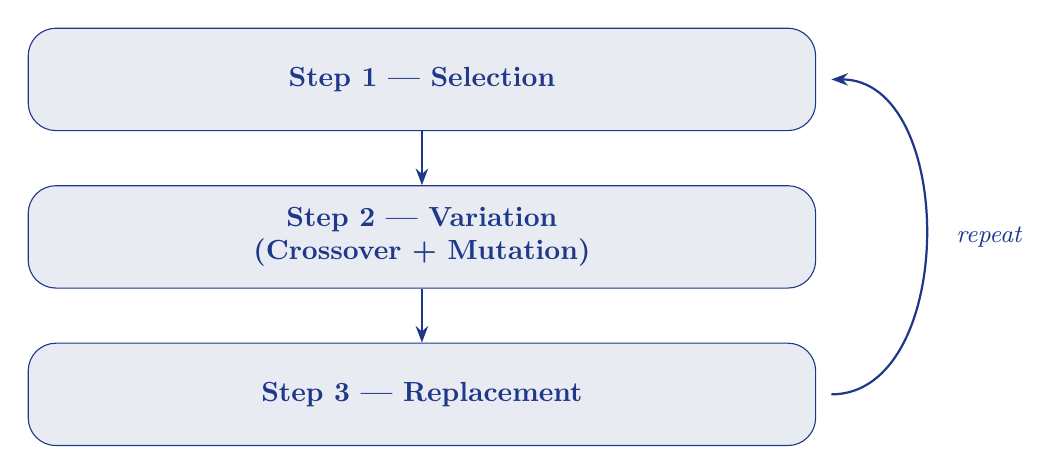
\begin{tikzpicture}[
  pill/.style={
    draw=NavyBlue,
    fill=NavyBlue!10,
    rounded corners=10pt,
    minimum width=10cm,
    minimum height=1.3cm,
    align=center,
    font=\bfseries,
    text=NavyBlue
  },
  sub/.style={
    font=\small,
    text width=9cm,
    align=center
  }
]

% ---------------- STEP 1 ----------------
\onslide<1->{
\node[pill] (s1) at (0,3.0)
{Step 1 — Selection};

% \node[sub] at (0,2.3)
% {Choose promising parents based on objective values.};
}

% ---------------- STEP 2 ----------------
\onslide<2->{
\node[pill] (s2) at (0,1.0)
{Step 2 — Variation \\ (Crossover + Mutation)};

% \node[sub] at (0,0.3)
% {Crossover + Mutation \\
% Generate new candidate solutions.};

\draw[-{Stealth[length=6pt]}, thick, NavyBlue]
(s1.south) -- (s2.north);
}

% ---------------- STEP 3 ----------------
\onslide<3->{
\node[pill] (s3) at (0,-1.0)
{Step 3 — Replacement};

% \node[sub] at (0,-1.7)
% {Insert better offspring. Keep population size fixed.};

\draw[-{Stealth[length=6pt]}, thick, NavyBlue]
(s2.south) -- (s3.north);
}

% ---------------- REPEAT LOOP ----------------
\onslide<4->{
\draw[-{Stealth[length=6pt]}, thick, NavyBlue]
(5.2,-1.0) .. controls +(1.6,0) and +(1.6,0) .. (5.2,3.0);

\node[font=\small\itshape, text=NavyBlue]
at (7.2,1.0) {repeat};
}

\end{tikzpicture}
\end{center}

\end{frame}


%% ============================================================
%% SLIDE 5 — Selection explained with analogy
%% ============================================================
\begin{frame}{Step 1 in Detail: Selection}

  \begin{columns}[T]
    \column{0.50\textwidth}

    \begin{block}{What is Selection?}
      We look at every solution in the population and give
      \textbf{better-scoring solutions a higher chance} of being chosen
      as parents. Worse solutions can still be chosen — just less often.
    \end{block}


    \vspace{0.1em}
    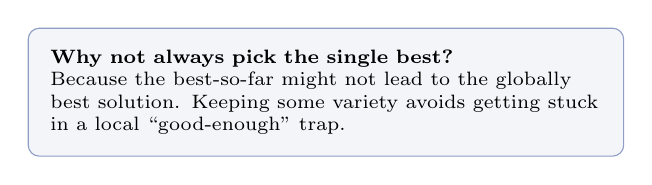
\begin{tikzpicture}
      \node[draw=NavyBlue!50, fill=NavyBlue!5, rounded corners=4pt,
            font=\scriptsize, inner sep=8pt, text width=7cm]
        {\textbf{Why not always pick the single best?}\\
         Because the best-so-far might not lead to the
         globally best solution. Keeping some variety avoids getting
         stuck in a local ``good-enough'' trap.};
    \end{tikzpicture}

    \column{0.47\textwidth}
    \begin{center}
    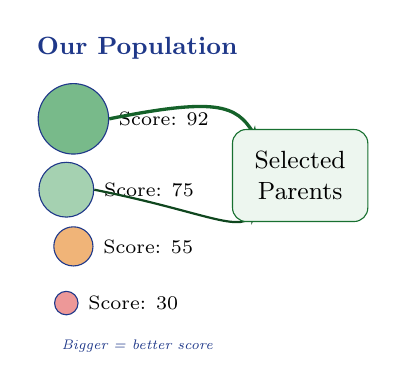
\begin{tikzpicture}[scale=0.9]
      % Population of 6 solutions as circles, sized by fitness
      \node[font=\small\bfseries, NavyBlue] at (1.5, 3.8) {Our Population};

      % solution nodes — size hints quality
      \node[circle, draw=NavyBlue, fill=GreenOK!60, inner sep=9pt,
            label={[font=\scriptsize]right:Score: 92}]   (A) at (0.6, 2.8) {};
      \node[circle, draw=NavyBlue, fill=GreenOK!40, inner sep=7pt,
            label={[font=\scriptsize]right:Score: 75}]   (B) at (0.5, 1.8) {};
      \node[circle, draw=NavyBlue, fill=CarOrange!60, inner sep=5pt,
            label={[font=\scriptsize]right:Score: 55}]   (C) at (0.6, 1.0) {};
      \node[circle, draw=NavyBlue, fill=CarRed!50, inner sep=3pt,
            label={[font=\scriptsize]right:Score: 30}]   (D) at (0.5, 0.2) {};

      % selection arrows from top two
      \draw[-{Stealth[length=5pt]}, GreenOK!70!black, very thick]
            (A.east) .. controls +(1.5,0.3) and +(-0.3,0.5) .. (3.2, 2.5);
      \draw[-{Stealth[length=5pt]}, GreenOK!50!black, thick]
            (B.east) .. controls +(1.5,-0.3) and +(-0.3,-0.3) .. (3.2, 1.5);

      % "selected parents" box
      \node[draw=GreenOK!80!black, fill=GreenOK!8, rounded corners=5pt,
            font=\small, inner sep=8pt, align=center] at (3.8, 2.0)
            {Selected\\Parents};

      \node[font=\tiny\itshape, text=NavyBlue] at (1.5, -0.4)
            {Bigger = better score};
    \end{tikzpicture}
    \end{center}
  \end{columns}
\end{frame}


%% ============================================================
%% SLIDE 6 — Crossover explained with analogy
%% ============================================================
\begin{frame}{Step 2a: Crossover — Mixing Parents}

  \begin{block}{What is Crossover?}
    Take \textbf{two parent solutions} and combine parts of each to
    create a \textbf{child solution}. The child gets some traits from
    Parent A and some from Parent B.
  \end{block}

  \vspace{0.4em}

  \begin{center}
  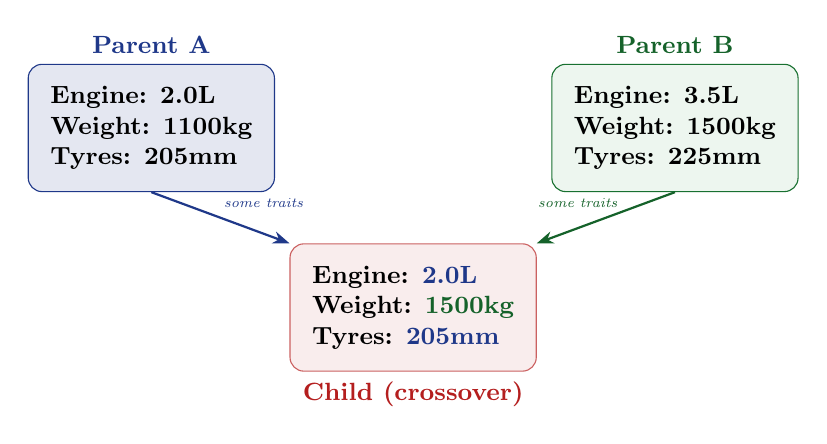
\begin{tikzpicture}[scale=0.95]

    % Parent A
    \node[draw=NavyBlue, fill=NavyBlue!12, rounded corners=5pt,
          font=\small\bfseries, inner sep=8pt, align=left,
          label={[font=\small\bfseries, NavyBlue]above:Parent A}]
          (PA) at (-3.5, 0)
          {Engine: 2.0L\\Weight: 1100kg\\Tyres: 205mm};

    % Parent B
    \node[draw=GreenOK!80!black, fill=GreenOK!8, rounded corners=5pt,
          font=\small\bfseries, inner sep=8pt, align=left,
          label={[font=\small\bfseries, GreenOK!70!black]above:Parent B}]
          (PB) at (3.5, 0)
          {Engine: 3.5L\\Weight: 1500kg\\Tyres: 225mm};

    % Child
    \node[draw=AlertRed!70, fill=AlertRed!8, rounded corners=5pt,
          font=\small\bfseries, inner sep=8pt, align=left,
          label={[font=\small\bfseries, AlertRed]below:Child (crossover)}]
          (CH) at (0, -2.4)
          {Engine: \textcolor{NavyBlue}{2.0L}\\
           Weight: \textcolor{GreenOK!70!black}{1500kg}\\
           Tyres: \textcolor{NavyBlue}{205mm}};

    % Arrows
    \draw[-{Stealth[length=6pt]}, NavyBlue, thick] (PA.south) -- (CH.north west);
    \draw[-{Stealth[length=6pt]}, GreenOK!70!black, thick] (PB.south) -- (CH.north east);

    % Labels on arrows
    \node[font=\tiny\itshape, NavyBlue] at (-2.0,-1.0) {some traits};
    \node[font=\tiny\itshape, GreenOK!70!black] at (2.2,-1.0) {some traits};
  \end{tikzpicture}
  \end{center}

  \vspace{0.2em}
  \begin{center}
    {\small\itshape The child might combine the best aspects of both parents —
    or produce something new entirely!}
  \end{center}
\end{frame}


%% ============================================================
%% SLIDE 7 — Mutation explained
%% ============================================================
\begin{frame}{Step 2b: Mutation — Adding a Little Randomness}

  \begin{columns}[T]
    \column{0.50\textwidth}

    \begin{block}{What is Mutation?}
      After crossover, we \textbf{randomly change} one or a few values
      in the child solution by a small amount.
    \end{block}

    \vspace{0.4em}
    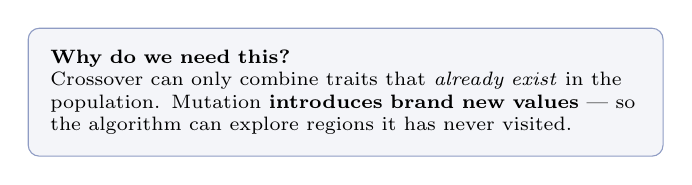
\begin{tikzpicture}
      \node[draw=NavyBlue!50, fill=NavyBlue!5, rounded corners=4pt,
            font=\scriptsize, inner sep=8pt, text width=7.5cm]
        {\textbf{Why do we need this?}\\
    Crossover can only combine traits that \emph{already exist} in the
    population. Mutation \textbf{introduces brand new values} — so the
    algorithm can explore regions it has never visited.};
    \end{tikzpicture}

    \column{0.47\textwidth}
    \begin{center}
    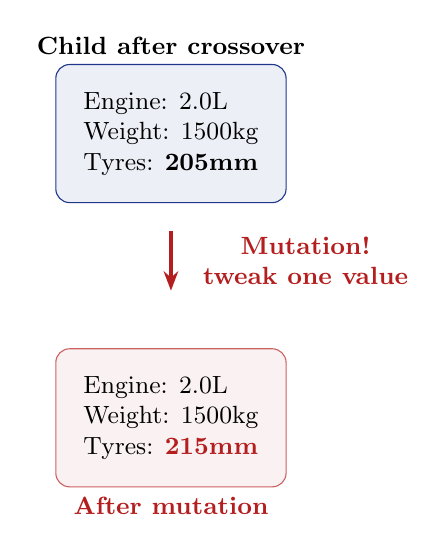
\begin{tikzpicture}[scale=0.95]
      % Before mutation box
      \node[draw=NavyBlue, fill=NavyBlue!8, rounded corners=5pt,
            font=\small, inner sep=10pt, align=left,
            label={[font=\small\bfseries]above:Child after crossover}]
            (bef) at (0, 1.8)
            {Engine: 2.0L\\Weight: 1500kg\\Tyres: \textbf{205mm}};

      % mutation arrow
      \draw[-{Stealth[length=7pt]}, AlertRed, very thick] (0,0.5) -- (0,-0.3);
      \node[font=\small\bfseries, AlertRed, align=center] at (1.8, 0.1)
            {Mutation!\\tweak one value};

      % After mutation box
      \node[draw=AlertRed!70, fill=AlertRed!6, rounded corners=5pt,
            font=\small, inner sep=10pt, align=left,
            label={[font=\small\bfseries, AlertRed]below:After mutation}]
            (aft) at (0,-2.0)
            {Engine: 2.0L\\Weight: 1500kg\\Tyres: \textbf{\textcolor{AlertRed}{215mm}}};

    \end{tikzpicture}
    \end{center}
  \end{columns}
\end{frame}


%% ============================================================
%% SLIDE 9 — Animated Simulation (population cloud moving)
%% ============================================================
\begin{frame}{Let's Watch It Happen: A Visual Simulation}

  \begin{columns}[c]
    \column{0.62\textwidth}
    \begin{center}
    \begin{tikzpicture}[scale=0.88]

      % Axes
      \draw[-{Stealth}, thick, NavyBlue] (0,0)--(5.6,0);
      \draw[-{Stealth}, thick, NavyBlue] (0,0)--(0,4.6);
      \node[font=\small, NavyBlue] at (2.8,-0.4) {Fuel Use (less is better $\leftarrow$)};
      \node[font=\small, NavyBlue, rotate=90] at (-0.55, 2.3) {Speed (more is better $\uparrow$)};

      % Ideal corner shading
      \fill[GreenOK!12] (0,3.0) rectangle (1.8,4.4);
      \node[font=\tiny, text=GreenOK!70!black] at (1.0, 4.3) {ideal region};

      %% === Gen 0: random scattered cloud ===
      \only<1>{
        \node[font=\small\bfseries, NavyBlue] at (3.0, 5.5)
              {Generation 0 — random start};
        \foreach \x/\y in {4.1/0.8, 4.6/1.2, 3.8/0.5, 5.0/1.0, 4.3/1.8,
                            3.5/0.9, 4.7/0.6, 3.2/1.5, 4.9/1.4, 3.0/0.7}
          \node[circle, fill=CarGray!80, draw=gray!60, inner sep=3pt] at (\x,\y) {};
        \node[font=\scriptsize\itshape, text=gray] at (4.0, 5.1)
              {All solutions are poor — scattered with high fuel use, low speed};
      }

      %% === Gen 1: shift begins ===
      \only<2>{
        \node[font=\small\bfseries, NavyBlue] at (3.0, 5.5)
              {Generation 1 — first improvement};
        % old (faded)
        \foreach \x/\y in {4.1/0.8, 4.6/1.2, 3.8/0.5, 5.0/1.0, 4.3/1.8}
          \node[circle, fill=CarGray!25, draw=gray!20, inner sep=3pt] at (\x,\y) {};
        % new (blue)
        \foreach \x/\y in {3.4/1.4, 3.0/1.8, 3.6/2.2, 2.8/1.2, 3.2/2.6,
                            2.5/1.6, 3.8/2.0, 2.2/2.2, 3.0/2.8, 2.6/2.0}
          \node[circle, fill=CarBlue!80, draw=NavyBlue!60, inner sep=3pt] at (\x,\y) {};
        \node[font=\scriptsize\itshape, text=NavyBlue] at (3.5, -1.0)
              {Selection + crossover pulled the cloud toward better regions};
      }

      %% === Gen 2: approaching front ===
      \only<3>{
        \node[font=\small\bfseries, NavyBlue] at (3.0, 5.5)
              {Generation 2 — converging fast};
        % faded gen1
        \foreach \x/\y in {3.4/1.4, 3.0/1.8, 3.6/2.2, 2.8/1.2}
          \node[circle, fill=CarGray!25, draw=gray!20, inner sep=3pt] at (\x,\y) {};
        % new (green)
        \foreach \x/\y in {1.8/2.6, 1.4/3.0, 2.2/3.2, 1.0/3.5,
                            1.6/3.4, 0.8/3.7, 2.0/3.0, 1.2/3.2, 1.9/2.8, 0.6/3.8}
          \node[circle, fill=GreenOK!75, draw=GreenOK!60!black, inner sep=3pt]
                at (\x,\y) {};
        % dashed emerging front
        \draw[AlertRed, dashed, thick]
              (0.4,3.9) .. controls (1.0,3.4) .. (2.0,2.8)
              .. controls (2.8,2.0) .. (3.8,1.0);
        \node[font=\tiny\bfseries, AlertRed, rotate=-42] at (2.0,1.7)
              {front emerging};
      }

      %% === Converged ===
      \only<4>{
        \node[font=\small\bfseries, NavyBlue] at (3.0, 5.5)
              {Converged — Pareto Front Discovered!};
        % interior faded
        \foreach \x/\y in {1.8/2.2, 2.2/1.8, 2.5/2.5}
          \node[circle, fill=CarGray!20, draw=gray!15, inner sep=3pt] at (\x,\y) {};
        % front points
        \foreach \x/\y in {0.3/3.9, 0.7/3.7, 1.1/3.4, 1.5/3.1,
                            1.9/2.8, 2.4/2.3, 2.9/1.7, 3.4/1.1, 3.9/0.6}
          \node[circle, fill=AlertRed!80, draw=AlertRed!70!black, inner sep=3.5pt]
                at (\x,\y) {};
        % front curve
        \draw[AlertRed, ultra thick]
              (0.3,3.9) .. controls (1.2,3.3) .. (2.0,2.7)
              .. controls (2.7,2.0) .. (3.9,0.6);
        \node[font=\small\bfseries, AlertRed, rotate=-42] at (2.0,1.8)
              {Pareto Front};
      }

    \end{tikzpicture}
    \end{center}

    \column{0.35\textwidth}
    \only<1>{
      \begin{block}{Generation 0}
        We \textbf{start randomly}. Most solutions are bad —
        high fuel use and low speed. But we have a wide spread to work with.
      \end{block}
      \vspace{0.3em}
      \small The gray dots are our initial population, scattered with no structure.
    }
    \only<2>{
      \begin{block}{Generation 1}
        \textbf{Selection} chose the slightly-better parents.
        \textbf{Crossover} mixed them. The whole cloud has \emph{shifted}
        toward lower fuel use and higher speed.
      \end{block}
    }
    \only<3>{
      \begin{block}{Generation 2}
        The population has \textbf{gathered near the frontier}.
        A Pareto front is beginning to take shape — diverse
        trade-off solutions are appearing.
      \end{block}
    }
    \only<4>{
      \begin{block}{Done!}
        After many generations we have a \textbf{full spread of
        non-dominated solutions} — the Pareto Front.
        Each red dot is a valid, excellent trade-off.
      \end{block}
      \vspace{0.3em}
      \alert{No single ``winner'' — the decision-maker chooses
      which trade-off fits their needs.}
    }

  \end{columns}
\end{frame}


%% ============================================================
%% SLIDE 10 — Why EAs are perfect for multi-objective problems
%% ============================================================
\begin{frame}{Why Is This Perfect for Multi-Objective Problems?}

  \begin{block}{Recall: In a multi-objective problem there is no single ``best'' — there is a \emph{set} of best trade-offs (the Pareto Front).}
  \end{block}

  \vspace{0.4em}

  \begin{columns}[T]
    \column{0.48\textwidth}
    \textbf{Classical optimisers find \emph{one} solution}
    \begin{center}
    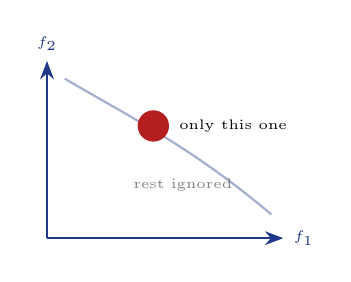
\begin{tikzpicture}[scale=0.75]
      \draw[-{Stealth}, NavyBlue, thick] (0,0)--(4,0) node[right,font=\tiny]{$f_1$};
      \draw[-{Stealth}, NavyBlue, thick] (0,0)--(0,3) node[above,font=\tiny]{$f_2$};
      \draw[NavyBlue!40, thick]
            (0.3,2.7) .. controls (1.5,2.0) and (2.5,1.5) .. (3.8,0.4);
      % Only one result
      \node[circle, fill=AlertRed, inner sep=4pt,
            label={[font=\tiny]right:only this one}] at (1.8,1.9) {};
      \node[font=\tiny, text=gray] at (2.3,0.9) {rest ignored};
    \end{tikzpicture}
    \end{center}
    \small They require you to \emph{decide} on a weighting up front.
    If priorities change, you must re-run from scratch.

    \column{0.48\textwidth}
    \textbf{EAs naturally find \emph{many} solutions}
    \begin{center}
    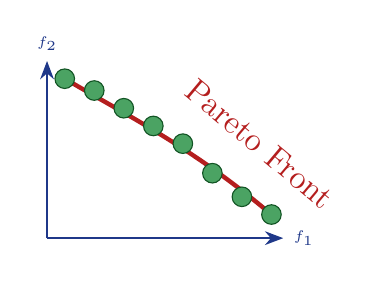
\begin{tikzpicture}[scale=0.75]
      \draw[-{Stealth}, NavyBlue, thick] (0,0)--(4,0) node[right,font=\tiny]{$f_1$};
      \draw[-{Stealth}, NavyBlue, thick] (0,0)--(0,3) node[above,font=\tiny]{$f_2$};
      \draw[AlertRed, ultra thick]
            (0.3,2.7) .. controls (1.5,2.0) and (2.5,1.5) .. (3.8,0.4);
      \node[font=\large, text=AlertRed, rotate=-40] at (3.6,1.6) {Pareto Front};
      \foreach \x/\y in {0.3/2.7, 0.8/2.5, 1.3/2.2, 1.8/1.9,
                          2.3/1.6, 2.8/1.1, 3.3/0.7, 3.8/0.4}
        \node[circle, fill=GreenOK!80, draw=GreenOK!60!black, inner sep=2.5pt]
              at (\x,\y) {};
    \end{tikzpicture}
    \end{center}
    \small The \textbf{population} maps naturally to a \emph{set} of trade-off solutions.
    One run gives the full picture.
  \end{columns}

  \vspace{0.4em}
  \begin{center}
    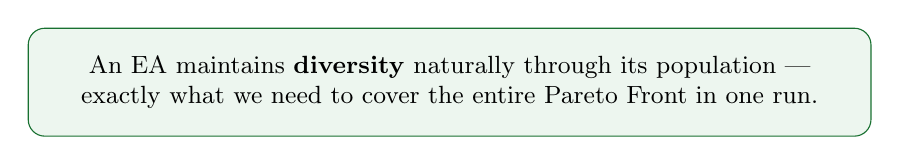
\begin{tikzpicture}
      \node[draw=GreenOK!80!black, fill=GreenOK!8, rounded corners=6pt,
            font=\small, inner sep=10pt, text width=10cm, text centered]
        {An EA maintains \textbf{diversity} naturally through its population
         — exactly what we need to cover the entire Pareto Front in one run.};
    \end{tikzpicture}
  \end{center}
\end{frame}


%% ============================================================
%% SLIDE 11 — Transition to MOEA/D
%% ============================================================
% \begin{frame}{So\ldots\ Where Does MOEA/D Come In?}

%   \begin{center}
%   \begin{tikzpicture}[
%     box/.style={draw=NavyBlue, fill=NavyBlue!10, rounded corners=8pt,
%                 minimum width=4.0cm, minimum height=1.4cm,
%                 align=center, font=\small\bfseries, text=NavyBlue,
%                 inner sep=8pt},
%     plus/.style={font=\Large\bfseries, NavyBlue},
%     result/.style={draw=GreenOK!80!black, fill=GreenOK!10, rounded corners=8pt,
%                    minimum width=9.5cm, minimum height=1.5cm,
%                    align=center, font=\bfseries, text=GreenOK!60!black,
%                    inner sep=10pt}
%   ]

%     \node[box] (ea)  at (-2.8, 0.5) {Evolutionary\\Algorithm\\(what we just learned)};
%     \node[plus]      at ( 0.0, 0.5) {$+$};
%     \node[box] (dec) at ( 2.8, 0.5)
%           {Decomposition\\(split the problem into\\many smaller sub-problems)};

%     \node[result] at (0, -1.6)
%           {MOEA/D — Solves all sub-problems simultaneously using the EA loop};

%     \draw[-{Stealth[length=6pt]}, GreenOK!70!black, thick]
%           (ea.south)  .. controls +(0,-0.6) and +(-2,0) .. (-1.2,-1.0);
%     \draw[-{Stealth[length=6pt]}, GreenOK!70!black, thick]
%           (dec.south) .. controls +(0,-0.6) and +( 2,0) .. ( 1.2,-1.0);
%   \end{tikzpicture}
%   \end{center}

%   \vspace{0.3em}

%   \begin{columns}[T]
%     \column{0.48\textwidth}
%     \textbf{What you now understand:}
%     \begin{itemize}
%       \item Solutions are candidates that get scored
%       \item Selection, crossover, mutation drive improvement
%       \item A population naturally explores many trade-offs
%     \end{itemize}

%     \column{0.48\textwidth}
%     \textbf{What MOEA/D adds:}
%     \begin{itemize}
%       \item Each solution ``owns'' a direction in objective space
%       \item Neighbouring solutions help each other improve
%       \item This makes the search much more \textbf{structured and efficient}
%     \end{itemize}
%   \end{columns}

%   \vspace{0.4em}
%   \begin{center}
%     \begin{tikzpicture}
%       \node[draw=NavyBlue!50, fill=NavyBlue!5, rounded corners=5pt,
%             font=\small\itshape, inner sep=8pt, text width=9.5cm, text centered]
%         {``Decompose the multi-objective problem into many scalar
%           sub-problems and solve them simultaneously.''\\[0.3em]
%          \normalfont\scriptsize --- Zhang \& Li, 2007};
%     \end{tikzpicture}
%   \end{center}
% \end{frame}




%% ============================================================
%% EVOLUTIONARY ALGORITHM SLIDES — BEGINNER FRIENDLY VERSION
%% Insert these slides AFTER the Summary frame, BEFORE


%% ============================================================
%% PART 2: DECOMPOSITION & WEIGHT VECTORS (Speaker 2 — Fathum Mobin)
%% ============================================================
% =============================================================================
% TITLE AND INTRODUCTION
% =============================================================================
\begin{frame}{MOEA/D: The Idea of Decomposition}
\begin{center}

\vspace{0.6em}
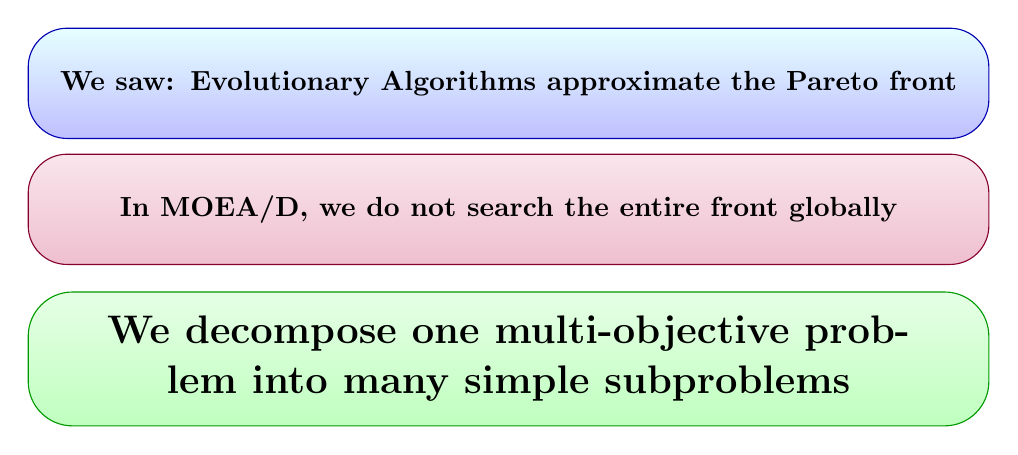
\begin{tikzpicture}

% -------- Top context box --------
\node[
draw=blue!70!black,
rounded corners=14pt,
top color=cyan!10,
bottom color=blue!25,
minimum width=12.2cm,
minimum height=1.4cm,
text width=11.8cm,
align=center,
font=\normalsize\bfseries
] at (0,2.1)
{We saw: Evolutionary Algorithms approximate the Pareto front};

% -------- Middle statement box --------
\node[
draw=purple!70!black,
rounded corners=14pt,
top color=purple!10,
bottom color=purple!25,
minimum width=12.2cm,
minimum height=1.4cm,
text width=11.8cm,
align=center,
font=\normalsize\bfseries
] at (0,0.5)
{In MOEA/D, we do not search the entire front globally};

% -------- Key idea box --------
\node[
draw=green!60!black,
rounded corners=16pt,
top color=green!10,
bottom color=green!25,
minimum width=12.2cm,
minimum height=1.7cm,
text width=11.8cm,
align=center,
font=\Large\bfseries
] at (0,-1.4)
{We decompose one multi-objective problem into many simple subproblems};

\end{tikzpicture}

\end{center}
\end{frame}



\begin{frame}{The Idea of Decomposition}
\begin{center}

\vspace{0.7em}

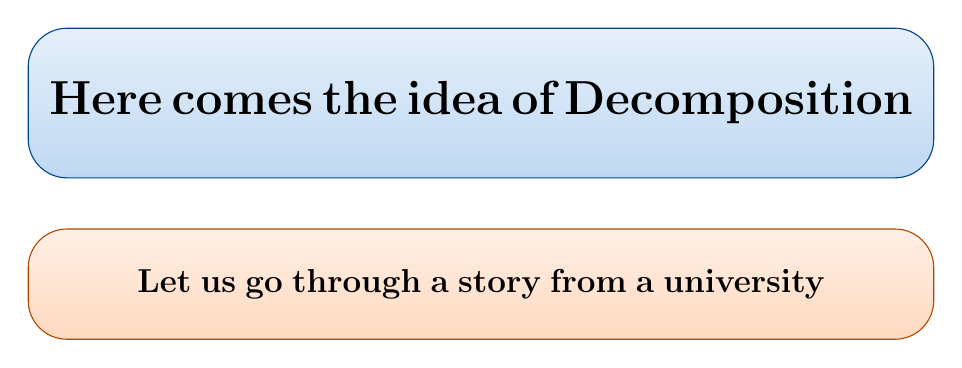
\begin{tikzpicture}

% -------- Top box (MAIN, bigger) --------
\node[
draw=maincolor!70!black,
rounded corners=14pt,
top color=maincolor!10,
bottom color=maincolor!25,
minimum width=11.5cm,
minimum height=1.9cm,
text width=11.0cm,
align=center
] at (0,1.4)
{{\LARGE\bfseries Here comes the idea of Decomposition}};

% -------- Bottom box (smaller) --------
\node[
draw=accentcolor!70!black,
rounded corners=14pt,
top color=accentcolor!10,
bottom color=accentcolor!25,
minimum width=11.5cm,
minimum height=1.4cm,
text width=11.0cm,
align=center
] at (0,-0.9)
{{\large\bfseries Let us go through a story from a university}};

\end{tikzpicture}

\end{center}
\end{frame}
% ------ Slide 1: Scene Setting ------
\begin{frame}{It's That Time of Year...}
\begin{center}

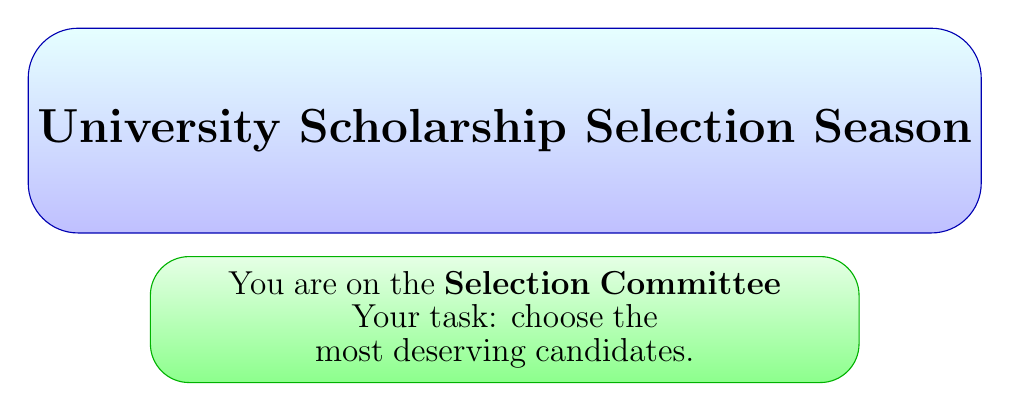
\begin{tikzpicture}

% -------- Main title card (forced single line) --------
\node[
draw=blue!70!black,
rounded corners=18pt,
top color=cyan!10,
bottom color=blue!25,
minimum width=11.2cm,
minimum height=2.6cm,
align=center
] at (0,0.4)
{{\LARGE\bfseries University Scholarship Selection Season}};

% -------- Role box --------
\node[
draw=green!70!black,
rounded corners=14pt,
top color=green!10,
bottom color=green!45,
minimum width=9.0cm,
minimum height=1.6cm,
text width=8.5cm,
align=center
] at (0,-2.0)
{{\large You are on the \textbf{Selection Committee}\\
Your task: choose the most deserving candidates.}};

\end{tikzpicture}

\end{center}
\end{frame}


% ------ Slide 2: The Stack ------
\begin{frame}{The Stack on Your Desk}
\begin{center}
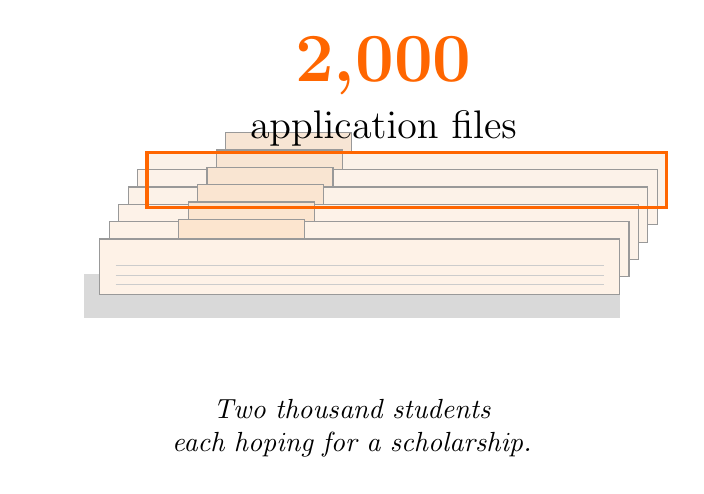
\begin{tikzpicture}

% Shadow
\fill[black!15] (-3.4,-0.3) rectangle (3.4,0.25);

% File stack
\foreach \i in {5,4,3,2,1,0} {

  % Folder body
  \filldraw[
    draw=black!40,
    fill=brown!\the\numexpr 20+\i*8\relax!orange!10
  ]
  (\i*0.12-3.2, \i*0.22)
  rectangle ++(6.6,0.7);

  % Folder tab
  \filldraw[
    draw=black!40,
    fill=brown!\the\numexpr 25+\i*8\relax!orange!20
  ]
  (\i*0.12-2.2, \i*0.22+0.7)
  rectangle ++(1.6,0.25);

  % Paper lines inside (top 2 folders only for realism)
  \ifnum\i<2
    \foreach \y in {0.12,0.24,0.36} {
      \draw[black!20] (\i*0.12-3.0, \i*0.22+\y) -- ++(6.2,0);
    }
  \fi
}

% Highlight top file border
\draw[accentcolor, line width=1.2pt]
(5*0.12-3.2,5*0.22) rectangle ++(6.6,0.7);

% Big number (moved higher)
\node[
  font=\fontsize{42}{42}\bfseries,
  text=accentcolor
] at (0.4,2.9) {2,000};

% Subtitle (now above the stack)
\node[
  font=\Large,
  text=black
] at (0.4,2.1) {application files};

% Caption
\node[
  font=\normalsize\itshape,
  text width=8cm,
  align=center
] at (0, -1.7)
{Two thousand students\\
each hoping for a scholarship.};

\end{tikzpicture}
\end{center}
\end{frame}

% ------ Slide 3: Meet the Applicants ------
\begin{frame}{You Open the First Few Files...}
\begin{center}
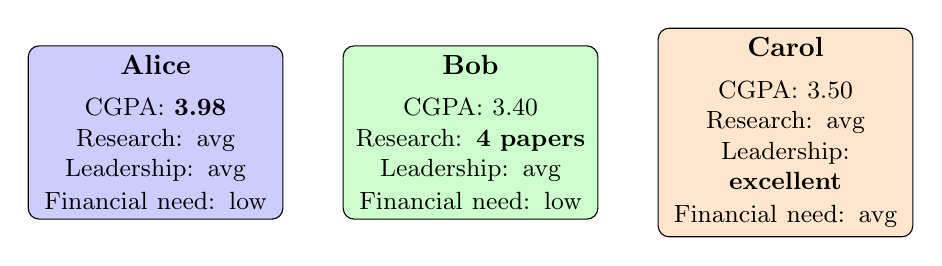
\begin{tikzpicture}[
  card/.style={draw, rounded corners, fill=#1, minimum width=3.2cm,
               minimum height=2.2cm, text width=3cm, align=center}]

  \node[card=blue!20]   at (0,   0) {\textbf{Alice}\\[0.4em]
                                      \small CGPA: \textbf{3.98}\\
                                      Research: avg\\
                                      Leadership: avg\\
                                      Financial need: low};

  \node[card=green!20]  at (4,   0) {\textbf{Bob}\\[0.4em]
                                      \small CGPA: 3.40\\
                                      Research: \textbf{4 papers}\\
                                      Leadership: avg\\
                                      Financial need: low};

  \node[card=orange!20] at (8,   0) {\textbf{Carol}\\[0.4em]
                                      \small CGPA: 3.50\\
                                      Research: avg\\
                                      Leadership: \textbf{excellent}\\
                                      Financial need: avg};
\end{tikzpicture}
\end{center}
\end{frame}


% ------ Slide 4: And More... ------
\begin{frame}{...And More Files}
\begin{center}

\begin{tikzpicture}[
  card/.style={draw, rounded corners, fill=#1, minimum width=3.2cm,
               minimum height=2.2cm, text width=3cm, align=center}]

  \node[card=red!20]    at (0,   0) {\textbf{Dave}\\[0.4em]
                                      \small CGPA: 3.10\\
                                      Research: low\\
                                      Leadership: avg\\
                                      Financial need: \textbf{very high}};

  \node[card=purple!15] at (4,   0) {\textbf{Eva}\\[0.4em]
                                      \small CGPA: 3.70\\
                                      Research: \textbf{3 papers}\\
                                      Leadership: \textbf{good}\\
                                      Financial need: avg};

  \node[font=\normalsize\itshape, text width=5cm, align=center] at (8, 0)
       {$\cdots$ and 1,995 more just like these.};

\end{tikzpicture}
\end{center}
\end{frame}


% ------ Slide 5: Naive Question ------
\begin{frame}{The Obvious Question}
\begin{center}
\vspace{1em}
{\LARGE \textbf{``JUST RANK THEM!!!''}}

\vspace{2em}
\begin{tikzpicture}
  \node[draw, rounded corners, fill=gray!10, minimum width=8cm,
        minimum height=1.5cm, text width=7.8cm, align=center, font=\large] at (0,0)
       {Assign a score to each applicant.\\
        Sort from best to worst. Pick the top ones.};
\end{tikzpicture}

\vspace{2em}
{\large Sounds simple, right?}
\end{center}
\end{frame}


% ------ Slide 6: But wait... ------
\begin{frame}{But Wait --- What's the Score?}
\begin{center}
\begin{tikzpicture}
  \node[font=\large, text width=10cm, align=center] at (0, 1.5)
       {To give a single score, you need to combine all four criteria.};

  \node[draw, rounded corners, fill=yellow!20, minimum width=9cm,
        minimum height=1.2cm, text width=8.8cm, align=center] at (0, 0)
       {\large $\text{score} = w_1 \cdot \text{CGPA} + w_2 \cdot \text{Research} + w_3 \cdot \text{Leadership} + w_4 \cdot \text{Need}$};

  \node[font=\large\bfseries, text=accentcolor] at (0, -1.5)
       {What should $w_1, w_2, w_3, w_4$ be?};
\end{tikzpicture}
\end{center}
\end{frame}


% ------ Slide 7: The Weight Problem ------
\begin{frame}{Nobody Agrees on the Weights}
\begin{center}
\begin{tikzpicture}[
bubble/.style={
draw=black!50,
rounded corners=10pt,
fill=#1,
minimum width=3.2cm,
minimum height=2.1cm,
text width=2.7cm,
align=center,
font=\small,
drop shadow
},
tail/.style={draw=black!50, fill=#1}
]

% -------- Prof A --------
\node[bubble=blue!15] (A) at (0,2)
{Prof.\ A:\\[0.2em]
\textit{``CGPA is everything!''}};
\draw[tail=blue!15] (-0.6,1.2) -- (-0.3,1.5) -- (-0.1,1.1) -- cycle;

% -------- Prof B --------
\node[bubble=green!15] (B) at (4.5,2)
{Prof.\ B:\\[0.2em]
\textit{``Research matters most.''}};
\draw[tail=green!15] (3.9,1.2) -- (4.2,1.5) -- (4.4,1.1) -- cycle;

% -------- Prof C --------
\node[bubble=orange!15] (C) at (0,-0.8)
{Prof.\ C:\\[0.2em]
\textit{``We need leaders!''}};
\draw[tail=orange!15] (-0.6,-1.6) -- (-0.3,-1.3) -- (-0.1,-1.7) -- cycle;

% -------- Prof D --------
\node[bubble=red!15] (D) at (4.5,-0.8)
{Prof.\ D:\\[0.2em]
\textit{``Financial need is priority.''}};
\draw[tail=red!15] (3.9,-1.6) -- (4.2,-1.3) -- (4.4,-1.7) -- cycle;

% -------- Right-side summary --------
\node[
font=\large\itshape,
text width=5.2cm,
align=center
] at (9.2,0.6)
{Every committee member has a \textbf{different} notion of ``best''.};

\end{tikzpicture}
\end{center}
\end{frame}


% ------ Slide 8: Try Anyway --- Compare Alice vs Bob ------
\begin{frame}{Okay, Let's Try. Who's Better: Alice or Bob?}
\begin{center}
\begin{tikzpicture}
  \node[draw, rounded corners, fill=blue!20, minimum width=3.5cm, minimum height=3cm,
        text width=3.3cm, align=center] (alice) at (0, 0)
       {\textbf{Alice}\\[0.5em]
        \small CGPA: \textcolor{blue}{\textbf{3.98}}\\
        Research: 0 papers\\
        Leadership: Avg\\
        Need: Low};

  \node[font=\LARGE\bfseries] at (4, 0) {vs};

  \node[draw, rounded corners, fill=green!20, minimum width=3.5cm, minimum height=3cm,
        text width=3.3cm, align=center] (bob) at (8, 0)
       {\textbf{Bob}\\[0.5em]
        \small CGPA: 3.40\\
        Research: \textcolor{green!60!black}{\textbf{4 papers}}\\
        Leadership: Avg\\
        Need: Low};

  \node[draw, rounded corners, fill=yellow!20, text width=6cm, align=center,
        font=\normalsize] at (4, -2.5)
       {Alice wins on CGPA.\\
        Bob wins on Research.\\
        \textbf{Nobody dominates the other.}};
\end{tikzpicture}
\end{center}
\end{frame}


% ------ Slide 9: Now scale it up ------
\begin{frame}{Now Do That for 2,000 Applicants}
\begin{center}
\begin{tikzpicture}[scale=1]

% ---- Mini applicant cards (grid) ----
\foreach \x in {0,0.8,...,5.6} {
  \foreach \y in {0,0.7,...,3.5} {
    \node[
      draw=black!30,
      fill=maincolor!15,
      rounded corners=2pt,
      minimum width=0.45cm,
      minimum height=0.55cm
    ] at (\x,\y) {};
  }
}

% ---- Light comparison mesh (background) ----
\foreach \a/\b in {0/0,1.6/1.4,3.2/2.1,4.8/0.7} {
  \foreach \c/\d in {0.8/2.8,2.4/0.7,4/3.5,5.6/1.4} {
    \draw[gray!20] (\a,\b) -- (\c,\d);
  }
}

% ---- Highlight a few comparisons ----
\draw[accentcolor, thick] (0,0) -- (2.4,0.7);
\draw[accentcolor, thick] (1.6,1.4) -- (4,3.5);
\draw[accentcolor, thick] (3.2,2.1) -- (5.6,1.4);

% ---- Arrow to explosion box ----
\draw[->, ultra thick, accentcolor] (6.2, 1.8) -- (7.7, 1.8);

% ---- Result box ----
\node[
draw=red!50,
rounded corners=6pt,
fill=red!15,
minimum width=3.8cm,
minimum height=2.1cm,
text width=3.4cm,
align=center,
font=\bfseries
] at (9.8, 1.8)
{$\approx 2{,}000{,}000$\\comparisons!};

% ---- Caption ----
\node[
font=\normalsize\itshape,
text width=9cm,
align=center
] at (4.5, -1.0)
{Every applicant must be compared with every other applicants.\\
Computationally expensive \textit{and} conceptually messy.};

\end{tikzpicture}
\end{center}
\end{frame}

% ------ Slide 10: Diversity Problem ------
\begin{frame}{And Even If You Do It...}
\begin{center}
\textbf{\large Final Top 10 Selected:}

\vspace{0.6em}
\begin{tikzpicture}
  % Row 1
  \node[draw, fill=blue!20, rounded corners, minimum width=2.8cm, font=\small,
        minimum height=0.65cm, text width=2.6cm, align=center] at (0*3.0, 1.2)
        {\#1 Alice\\\tiny CGPA: 3.98};
  \node[draw, fill=blue!20, rounded corners, minimum width=2.8cm, font=\small,
        minimum height=0.65cm, text width=2.6cm, align=center] at (1*3.0, 1.2)
        {\#2 James\\\tiny CGPA: 3.97};
  \node[draw, fill=blue!20, rounded corners, minimum width=2.8cm, font=\small,
        minimum height=0.65cm, text width=2.6cm, align=center] at (2*3.0, 1.2)
        {\#3 Priya\\\tiny CGPA: 3.96};
  \node[draw, fill=blue!20, rounded corners, minimum width=2.8cm, font=\small,
        minimum height=0.65cm, text width=2.6cm, align=center] at (3*3.0, 1.2)
        {\#4 Lena\\\tiny CGPA: 3.95};
  \node[draw, fill=blue!20, rounded corners, minimum width=2.8cm, font=\small,
        minimum height=0.65cm, text width=2.6cm, align=center] at (4*3.0, 1.2)
        {\#5 Omar\\\tiny CGPA: 3.94};
  % Row 2
  \node[draw, fill=blue!20, rounded corners, minimum width=2.8cm, font=\small,
        minimum height=0.65cm, text width=2.6cm, align=center] at (0*3.0, 0.2)
        {\#6 Sara\\\tiny CGPA: 3.93};
  \node[draw, fill=blue!20, rounded corners, minimum width=2.8cm, font=\small,
        minimum height=0.65cm, text width=2.6cm, align=center] at (1*3.0, 0.2)
        {\#7 Chen\\\tiny CGPA: 3.92};
  \node[draw, fill=blue!20, rounded corners, minimum width=2.8cm, font=\small,
        minimum height=0.65cm, text width=2.6cm, align=center] at (2*3.0, 0.2)
        {\#8 Fatima\\\tiny CGPA: 3.91};
  \node[draw, fill=blue!20, rounded corners, minimum width=2.8cm, font=\small,
        minimum height=0.65cm, text width=2.6cm, align=center] at (3*3.0, 0.2)
        {\#9 Ravi\\\tiny CGPA: 3.90};
  \node[draw, fill=blue!20, rounded corners, minimum width=2.8cm, font=\small,
        minimum height=0.65cm, text width=2.6cm, align=center] at (4*3.0, 0.2)
        {\#10 Nina\\\tiny CGPA: 3.89};

  \node[draw, rounded corners, fill=red!15, text width=11cm, align=center,
        font=\normalsize, minimum height=1.2cm] at (6.0, -1.5)
       {\textbf{Problem:} Every selected candidate has a high CGPA --- and nothing else.\\
        Bob (4 papers), Carol (leadership), Dave (financial need) --- all rejected.};
\end{tikzpicture}
\end{center}
\end{frame}


% ------ Slide 11: The Real Issue ------
\begin{frame}{The Real Issue}
\begin{center}
\vspace{0.5em}
\begin{tikzpicture}
  \node[draw, rounded corners, fill=accentcolor!15, minimum width=10cm,
        minimum height=1.5cm, text width=9.8cm, align=center, font=\large\bfseries] at (0, 1.5)
       {There is no single ``Best'' applicant.\\
        There are only applicants who are best \textit{in a certain way}.};

  \node[font=\normalsize, text width=9cm, align=center] at (0, -0.5)
       {\textbf{Alice} is best if you care about \textbf{CGPA}.\\
        \textbf{Bob} is best if you care about \textbf{Research}.\\
        \textbf{Dave} is best if you care about \textbf{Financial need}.};

  \node[font=\normalsize\itshape, text width=9cm, align=center] at (0, -2.3)
       {Forcing a single global ranking destroys this structure.};
\end{tikzpicture}
\end{center}
\end{frame}


% ------ Slide 12: A Better Idea Emerges ------
\begin{frame}{A Better Idea Starts to Form...}
\begin{center}

{\large What if we \textbf{stopped} trying to build one global ranking...}

\vspace{1.4em}

\begin{tikzpicture}

% -------- Top box: global ranking --------
\node[
draw=red!60!black,
line width=1pt,
rounded corners=8pt,
top color=red!10,
bottom color=red!25,
minimum width=9cm,
minimum height=1.3cm,
text width=8.4cm,
align=center,
font=\bfseries,
drop shadow
] (global) at (0,0)
{One hard global ranking\\
(expensive, unfair, not diverse)};

% Arrow
\draw[->, ultra thick, accentcolor] (0,-0.85) -- (0,-1.75);

% -------- Bottom box: decomposition idea --------
\node[
draw=successcolor!60!black,
line width=1pt,
rounded corners=8pt,
top color=successcolor!15,
bottom color=successcolor!30,
minimum width=9cm,
minimum height=1.3cm,
text width=8.4cm,
align=center,
font=\bfseries,
drop shadow
] (decomp) at (0,-2.6)
{Several focused sub-selections\\
(one per preference type)};

% Caption
\node[
font=\normalsize\itshape,
text width=8.5cm,
align=center
] at (0,-4.0)
{Each sub-problem is simple. Together, they cover everything.};

\end{tikzpicture}

\end{center}
\end{frame}


% ------ Slide 13: One Pattern Emerges ------



% ------ Slide 14: The Two Questions ------
\begin{frame}{Two Questions That Change Everything}
\begin{center}

\begin{tikzpicture}

% -------- Question 1 --------
\node[
draw=maincolor!70!black,
line width=1pt,
rounded corners=10pt,
top color=maincolor!10,
bottom color=maincolor!25,
minimum width=12cm,
minimum height=1.5cm,
align=center,
font=\large\bfseries,
drop shadow
] at (0,1.4)
{What if we stop building one global ranking?};

% -------- Question 2 --------
\node[
draw=accentcolor!70!black,
line width=1pt,
rounded corners=10pt,
top color=accentcolor!10,
bottom color=accentcolor!25,
minimum width=12cm,
minimum height=1.5cm,
align=center,
font=\large\bfseries,
drop shadow
] at (0,-0.6)
{What if we evaluate under different preferences instead?};

% -------- Caption --------
\node[
font=\normalsize\itshape,
text width=9cm,
align=center
] at (0,-2.8)
{These two questions lead us directly to the core idea behind \textbf{MOEA/D}.};

\end{tikzpicture}

\end{center}
\end{frame}



% =============================================================================
% STEP 1 — Preference-based Selection (continue scholarship story)
% =============================================================================



\begin{frame}{And Together, They Cover Everything}
\begin{center}
\begin{tikzpicture}[
  win/.style={draw, rounded corners, fill=#1, minimum width=4.5cm,
              minimum height=1.4cm, text width=4.3cm, align=center}]

  \node[win=blue!20]   at (0,   1.5) {\textbf{Bob} — Research\\{\small 4 publications}};
  \node[win=orange!20] at (5,   1.5) {\textbf{Carol} — Leadership\\{\small Club president, 3 NGOs}};
  \node[win=red!20]    at (0,  -0.3) {\textbf{Dave} — Need-Based\\{\small Family income: very low}};
  \node[win=purple!15] at (5,  -0.3) {\textbf{Eva} — Balanced\\{\small Good across all criteria}};

  \node[draw, rounded corners, fill=successcolor!20, text width=10cm, align=center,
        minimum height=1.0cm, font=\large\bfseries] at (2.5, -2.2)
       {Diverse. Fair. No single winner dominates.};
\end{tikzpicture}
\end{center}
\end{frame}


% =============================================================================
% STEP 2 — Insight Slide
% =============================================================================

\begin{frame}{The Key Insight}
\begin{center}
\begin{tikzpicture}
  \node[draw, rounded corners, fill=red!15, minimum width=9cm, minimum height=1.3cm,
        text width=8.8cm, align=center, font=\large\bfseries] at (0, 2)
       {One global ranking \quad $\boldsymbol{\times}$};

  \node[draw, rounded corners, fill=successcolor!20, minimum width=9cm, minimum height=1.3cm,
        text width=8.8cm, align=center, font=\large\bfseries] at (0, 0.2)
       {Multiple preference-based rankings \quad $\boldsymbol{\checkmark}$};

  \node[font=\normalsize, text width=8cm, align=center] at (0, -1.5)
       {Each sub-ranking is \textbf{simple} to compute.\\
        Together, they are \textbf{complete} — covering all preference directions.};
\end{tikzpicture}
\end{center}
\end{frame}


% =============================================================================
% STEP 3 — Map to Optimization + Introduce "Decomposition"
% =============================================================================




\begin{frame}{This Is Called: \textbf{Decomposition}}
\begin{center}

\vspace{0.4em}
{\LARGE Instead of one hard problem,}

\vspace{0.6em}
{\LARGE solve many simple ones.}

\vspace{1.2em}

\begin{tikzpicture}

% ---- Main Decomposition Box ----
\node[
draw=accentcolor!70!black,
line width=1pt,
rounded corners=10pt,
top color=accentcolor!10,
bottom color=accentcolor!25,
minimum width=11cm,
minimum height=1.5cm,
align=center,
font=\Large\bfseries,
drop shadow
] at (0,0)
{$\longrightarrow$ \quad Decomposition \quad $\longleftarrow$};

% ---- Definition Box ----
\node[
draw=maincolor!70!black,
line width=1pt,
rounded corners=8pt,
top color=maincolor!10,
bottom color=maincolor!20,
minimum width=11cm,
minimum height=1.2cm,
align=center,
font=\normalsize,
drop shadow
] at (0,-1.8)
{Breaking a multiobjective optimization problem\\
into multiple scalar subproblems, each with a different preference.};

\end{tikzpicture}

\vspace{1.1em}

{\normalsize One multiobjective problem \quad $\Rightarrow$ \quad many scalar subproblems}

\end{center}
\end{frame}


% =============================================================================
% STEP 4 — Visual Decomposition
% =============================================================================

\begin{frame}{Visualizing Decomposition}
\begin{center}
\begin{tikzpicture}[scale=0.95]

% ---- Hard problem box ----
\node[
draw=red!70!black,
line width=1pt,
rounded corners=8pt,
top color=red!10,
bottom color=red!25,
minimum width=4.8cm,
minimum height=1.6cm,
align=center,
font=\bfseries\large,
drop shadow
] (hard) at (0,2.5)
{One Hard\\Multiobjective Problem};

% ---- Arrow down ----
\draw[->, ultra thick, maincolor] (0,1.65) -- (0,0.9);
\node[font=\bfseries, text=maincolor] at (2.0,1.25) {Decompose};

% ---- Subproblem circles ----
\foreach \x/\g/\lbl in {
-4.6/g_1/Research focused,
-2.3/g_2/Leadership focused,
0/g_3/Balanced,
2.3/g_4/Need focused,
4.6/g_5/Academic focused}
{
\node[
draw=successcolor!70!black,
line width=0.9pt,
circle,
top color=successcolor!10,
bottom color=successcolor!30,
minimum size=1.25cm,
font=\bfseries,
drop shadow
] (\g) at (\x,-0.2) {$\g$};

\node[
font=\small,
text width=2.4cm,
align=center
] at (\x,-1.4) {\lbl};

\draw[->, thick, accentcolor] (0,0.9) -- (\g);
}

% ---- Bottom explanation box ----
\node[
draw=gray!60!black,
rounded corners=8pt,
top color=gray!5,
bottom color=gray!15,
minimum width=10.8cm,
minimum height=0.95cm,
align=center,
font=\normalsize,
drop shadow
] at (0,-2.6)
{Each $g_i$ is a \textbf{scalar} optimization problem — easy to solve individually.};

\end{tikzpicture}
\end{center}
\end{frame}


% =============================================================================
% PHONE STORY — Bridge from scholarship to objective space
% =============================================================================

\begin{frame}{A Second Story: Buying a Phone}
\begin{center}
\begin{tikzpicture}

% ---- Main card ----
\node[
draw=maincolor!70!black,
line width=1pt,
rounded corners=10pt,
top color=maincolor!10,
bottom color=maincolor!25,
minimum width=11cm,
minimum height=2.6cm,
align=center,
font=\Large\bfseries,
drop shadow
] at (0,0.2)
{You want to buy a new smartphone.};

% ---- Criteria text (manual line control, no awkward wrapping) ----
\node[
font=\normalsize,
align=center
] at (0,-2.0)
{You care about two things:\\[0.5em]
\textbf{1. Price} --- as low as possible \hspace{1.2cm}
\textbf{2. Camera Quality} --- as high as possible.};

\end{tikzpicture}
\end{center}
\end{frame}


\begin{frame}{You Walk Into the Store...}
\begin{center}
\begin{tikzpicture}[
phone/.style={
draw=#1!80!black,
line width=0.9pt,
rounded corners=10pt,
top color=#1!10,
bottom color=#1!25,
minimum width=3.4cm,
minimum height=3.1cm,
align=center,
font=\small,
drop shadow
}
]

% -------- Phone A --------
\node[phone=blue] at (0,0)
{\textbf{\large Phone A}\\[0.4em]
\textcolor{blue!70!black}{\textbf{\$200}}\\[0.3em]
Camera:\\
{\large\textbf{2/5}}\\[0.2em]
\tiny Budget pick};

% -------- Phone B --------
\node[phone=green!70!black] at (4.2,0)
{\textbf{\large Phone B}\\[0.4em]
\textbf{\$450}\\[0.3em]
Camera:\\
{\large\textbf{4/5}}\\[0.2em]
\tiny Mid-range};

% -------- Phone C --------
\node[phone=orange!80!black] at (8.4,0)
{\textbf{\large Phone C}\\[0.4em]
\textcolor{red!70!black}{\textbf{\$1{,}100}}\\[0.3em]
Camera:\\
{\large\textbf{5/5}}\\[0.2em]
\tiny Flagship};

% -------- Phone D --------
\node[phone=purple!70!black] at (12.6,0)
{\textbf{\large Phone D}\\[0.4em]
\textbf{\$500}\\[0.3em]
Camera:\\
{\large\textbf{2/5}}\\[0.2em]
\tiny Overpriced?};

\end{tikzpicture}
\end{center}
\end{frame}


\begin{frame}{Which One Is ``Best''?}
\begin{center}
\begin{tikzpicture}

% ---- Top statement ----
\node[
font=\large,
align=center
] at (0,2.1)
{It depends entirely on your \textbf{preference}.};

% ---- Budget winner ----
\node[
draw=blue!70!black,
line width=1pt,
rounded corners=10pt,
top color=blue!10,
bottom color=blue!25,
minimum width=5.6cm,
minimum height=1.3cm,
align=center,
font=\small\bfseries,
drop shadow
] at (-3.2,0.3)
{On a tight budget?\\Phone A wins};

% ---- Camera winner ----
\node[
draw=green!60!black,
line width=1pt,
rounded corners=10pt,
top color=green!10,
bottom color=green!25,
minimum width=5.6cm,
minimum height=1.3cm,
align=center,
font=\small\bfseries,
drop shadow
] at (3.2,0.3)
{Want the best camera?\\Phone C wins};

% ---- Balanced winner ----
\node[
draw=orange!80!black,
line width=1pt,
rounded corners=10pt,
top color=orange!10,
bottom color=orange!25,
minimum width=5.6cm,
minimum height=1.3cm,
align=center,
font=\small\bfseries,
drop shadow
] at (0,-1.2)
{Want a balance?\\Phone B wins};

% ---- Dominated phone ----
\node[
draw=gray!60,
rounded corners=10pt,
top color=gray!5,
bottom color=gray!15,
minimum width=10.5cm,
minimum height=1.1cm,
align=center,
font=\normalsize\itshape
] at (0,-2.7)
{And what about phone D? Phone D is dominated — nobody would choose it.};

\end{tikzpicture}
\end{center}
\end{frame}


\begin{frame}{Phone D Is Dominated}
\begin{center}
\begin{tikzpicture}[
phone/.style={
draw=#1!80!black,
line width=0.9pt,
rounded corners=10pt,
top color=#1!10,
bottom color=#1!25,
minimum width=3.6cm,
minimum height=2.3cm,
align=center,
font=\small,
drop shadow
}
]

% -------- Phone A --------
\node[phone=blue] (a) at (0,0)
{\textbf{Phone A}\\[0.3em]
\textbf{\$200}\\
cam 2/5};

% -------- Phone B --------
\node[phone=green!70!black] (b) at (6,0)
{\textbf{Phone B}\\[0.3em]
\textbf{\$450}\\
cam 4/5};

% -------- Phone D (dominated) --------
\node[
draw=gray!60,
rounded corners=10pt,
top color=gray!5,
bottom color=gray!15,
minimum width=3.6cm,
minimum height=2.3cm,
align=center,
font=\small
] (d) at (12,0)
{\textbf{Phone D}\\[0.3em]
\$500\\
cam 2/5};

% -------- Dominance arrow (lowered path) --------
\draw[->, ultra thick, red!70!black]
(b.east) -- ++(0.8,0) -- ++(0,-0.35) -- (d.west |- -0.35);

% -------- Arrow label (now fully clear) --------
\node[
font=\small\bfseries,
text=red!70!black,
align=center
] at (9,0.45)
{Better camera\\Lower price};

% -------- Bottom explanation box --------
\node[
draw=red!70!black,
rounded corners=10pt,
top color=red!10,
bottom color=red!25,
minimum width=12cm,
minimum height=1.1cm,
align=center,
font=\normalsize,
drop shadow
] at (6,-2.5)
{\textbf{Phone D is dominated.} Phone B is better in both criteria.\\
Dominated options can be safely ignored.};

\end{tikzpicture}
\end{center}
\end{frame}


\begin{frame}{The Phones That Remain: Non-Dominated}
\begin{center}
\begin{tikzpicture}[
phone/.style={
draw=#1!80!black,
line width=0.9pt,
rounded corners=10pt,
top color=#1!10,
bottom color=#1!25,
minimum width=3.2cm,
minimum height=2.0cm,
align=center,
font=\small,
drop shadow
}
]

% -------- Phone A --------
\node[phone=blue] (a) at (0,0)
{\textbf{Phone A}\\[0.3em]
\textbf{\$200}\\
cam 2/5\\
{\tiny Best price}};

% -------- Phone B --------
\node[phone=green!70!black] (b) at (6.5,0)
{\textbf{Phone B}\\[0.3em]
\textbf{\$450}\\
cam 4/5\\
{\tiny Balanced}};

% -------- Phone C --------
\node[phone=orange!80!black] (c) at (13,0)
{\textbf{Phone C}\\[0.3em]
\textbf{\$1{,}100}\\
cam 5/5\\
{\tiny Best camera}};

% -------- Non-dominance dashed links --------
\draw[<->, thick, gray!70, dashed] (a) -- (b);
\draw[<->, thick, gray!70, dashed] (b) -- (c);

% -------- Labels (now fully clear) --------
\node[font=\small\itshape, gray!80] at (3.25,1.0) {Neither dominates};
\node[font=\small\itshape, gray!80] at (9.75,1.0) {Neither dominates};

% -------- Pareto front explanation box --------
\node[
draw=successcolor!70!black,
rounded corners=10pt,
top color=successcolor!10,
bottom color=successcolor!25,
minimum width=13.5cm,
minimum height=1.2cm,
align=center,
font=\normalsize,
drop shadow
] at (6.5,-2.3)
{These three phones are \textbf{non-dominated} — the best trade-offs available.\\
Together they form the \textbf{PARETO FRONT}.};

\end{tikzpicture}
\end{center}
\end{frame}







% -----------------------------------------------------------------------
% SLIDE 32 — Back to phones: each preference = one subproblem
% -----------------------------------------------------------------------
\begin{frame}{Back to the Phone Store: Each Preference = One Subproblem}
\begin{center}
\begin{tikzpicture}[
  phone/.style={
    draw=black!35,
    rounded corners=10pt,
    top color=#1!8,
    bottom color=#1!18,
    minimum width=3.6cm,
    minimum height=2.6cm,
    align=center,
    font=\small
  },
  pref/.style={
    draw=black!35,
    rounded corners=10pt,
    fill=#1!15,
    minimum width=3.6cm,
    minimum height=1.1cm,
    align=center,
    font=\small\bfseries
  }
]

% -------- Phones --------
\node[phone=blue]  (pa) at (0, 0.6)
{\textbf{Phone A}\\[0.4em]
Price: \textcolor{blue}{\textbf{\$200}}\\
Camera: 2/5\\[0.2em]
{\tiny Best price}};

\node[phone=green] (pb) at (5, 0.6)
{\textbf{Phone B}\\[0.4em]
Price: \$450\\
Camera: \textcolor{green!60!black}{\textbf{4/5}}\\[0.2em]
{\tiny Balanced choice}};

\node[phone=orange] (pc) at (10, 0.6)
{\textbf{Phone C}\\[0.4em]
Price: \$1,100\\
Camera: \textcolor{orange!80!black}{\textbf{5/5}}\\[0.2em]
{\tiny Best camera}};

% -------- Preferences (NO text width, NO wrap possible) --------
\node[pref=blue]   (la) at (0,  -2.0)
{Budget focus\\$g_1$: minimize price};

\node[pref=green]  (lb) at (5,  -2.0)
{\mbox{Balanced preference}\\$g_3$: equal weight};

\node[pref=orange] (lc) at (10, -2.0)
{Camera focus\\$g_5$: \mbox{maximize quality}};

% -------- Arrows --------
\draw[->, thick, blue!60]   (pa.south) -- (la.north);
\draw[->, thick, green!60!black]  (pb.south) -- (lb.north);
\draw[->, thick, orange!80!black] (pc.south) -- (lc.north);

% -------- Bottom message --------
\node[
draw=black!40,
rounded corners=10pt,
fill=maincolor!10,
minimum width=12cm,
minimum height=0.9cm,
align=center,
font=\normalsize
] at (5, -3.4)
{Different preferences lead to different phones — and different scalar subproblems};

\end{tikzpicture}
\end{center}
\end{frame}


% -----------------------------------------------------------------------
% SLIDE 33 — Introducing the Weight Vector λ
% -----------------------------------------------------------------------
\begin{frame}{Introducing the Weight Vector $\lambda$}
\begin{center}
\begin{tikzpicture}[
  ex/.style={
    draw=black!35,
    rounded corners=10pt,
    top color=#1!10,
    bottom color=#1!25,
    minimum width=4.2cm,
    minimum height=1.6cm,
    text width=3.9cm,
    align=center,
    font=\normalsize
  }
]

% -------- Definition card --------
\node[
draw=maincolor!70!black,
rounded corners=12pt,
top color=maincolor!10,
bottom color=maincolor!25,
minimum width=11.2cm,
minimum height=1.6cm,
text width=10.8cm,
align=center,
font=\large\bfseries
] at (0,3.0)
{A weight vector $\lambda = (\lambda_1,\lambda_2)$\\
encodes a preference over objectives};

% -------- Constraint note --------
\node[font=\small, text=black!70] at (0,1.9)
{$\lambda_1 + \lambda_2 = 1 \quad (\text{like percentages})$};

% -------- Examples --------
\node[ex=blue] at (-4.4,0)
{$\lambda = (0.1,\,0.9)$\\[0.3em]
\small \textbf{Price-focused}\\"90\% Camera,\\ 10\% Price"\\
\tiny finds Phone C};

\node[ex=green] at (0,0)
{$\lambda = (0.5,\,0.5)$\\[0.3em]
\small \textbf{Perfectly Balanced}\\"50\% Camera,\\ 50\% Price"\\
\tiny finds Phone B};

\node[ex=orange] at (4.4,0)
{$\lambda = (0.9,\,0.1)$\\[0.3em]
\small \textbf{Camera-focused}\\"10\% Camera,\\ 90\% Price"\\
\tiny finds Phone A};

% -------- Key insight --------
\node[
draw=accentcolor!70!black,
rounded corners=12pt,
top color=accentcolor!10,
bottom color=accentcolor!25,
minimum width=11.2cm,
minimum height=1.2cm,
text width=10.8cm,
align=center,
font=\normalsize\bfseries
] at (0,-2.0)
{Each $\lambda$ defines one scalar subproblem\\
and one focused search direction};

\end{tikzpicture}
\end{center}
\end{frame}


% -----------------------------------------------------------------------
% SLIDE 34 — How Scalarization Works
% -----------------------------------------------------------------------
% \begin{frame}{How Do We Solve Each Sub-Problem? Scalarization}
% \begin{center}
% \begin{tikzpicture}[scale=0.95]

% % -------- Left: Multi-objective --------
% \node[
% draw=red!60!black,
% rounded corners=12pt,
% top color=red!10,
% bottom color=red!25,
% minimum width=4.6cm,
% minimum height=2.5cm,
% text width=4.3cm,
% align=center
% ] (mo) at (-3.6, 0)
% {{\bfseries Multi-objective}\\[0.5em]
% minimize $f_1$ and $f_2$\\[0.4em]
% {\small No single solution\\needs a full front}};

% % -------- Arrow --------
% \draw[->, ultra thick, maincolor!80]
% (-1.1,0) -- (1.1,0)
% node[above, midway, font=\small\bfseries, text=maincolor]
% {scalarize via $\lambda$};

% % -------- Right: Scalar --------
% \node[
% draw=successcolor!60!black,
% rounded corners=12pt,
% top color=successcolor!10,
% bottom color=successcolor!25,
% minimum width=4.6cm,
% minimum height=2.5cm,
% text width=4.3cm,
% align=center
% ] (sc) at (3.6, 0)
% {{\bfseries Scalar subproblem}\\[0.5em]
% minimize $g(\mathbf{f}\mid\lambda)$\\[0.4em]
% {\small One value to optimize\\simple and focused}};

% % -------- Explanation card --------
% \node[
% draw=maincolor!70!black,
% rounded corners=12pt,
% top color=maincolor!10,
% bottom color=maincolor!25,
% text width=10.8cm,
% align=center,
% minimum height=1.1cm,
% font=\normalsize
% ] at (0, -2.2)
% {The weight vector $\lambda$ converts multiple objectives\\into a \textbf{single score} based on a preference};

% % -------- Intuition quote --------
% \node[
% draw=black!40,
% rounded corners=10pt,
% fill=yellow!20,
% text width=10.2cm,
% align=center,
% minimum height=0.9cm,
% font=\small\itshape
% ] at (0, -3.4)
% {``Given my preference $\lambda$, what is the single score of this solution?''};

% \end{tikzpicture}
% \end{center}
% \end{frame}


% -----------------------------------------------------------------------
% SLIDE 35 — Two Classic Scalarization Methods
% -----------------------------------------------------------------------
\begin{frame}{Two Classic Ways to Scalarize}
\begin{center}
\begin{tikzpicture}[
  method/.style={
    draw=#1!70!black,
    rounded corners=12pt,
    top color=#1!10,
    bottom color=#1!25,
    minimum width=5.6cm,
    minimum height=3.6cm,
    text width=5.2cm,
    align=center
  }
]

% -------- Weighted Sum --------
\node[method=blue] (ws) at (0,0)
{{\bfseries\large Weighted Sum}\\[0.7em]
\small Combine objectives as\\a weighted average\\[0.5em]
{\footnotesize Score $= \lambda_1 f_1 + \lambda_2 f_2$}\\[0.6em]
{\footnotesize Simple \textbullet\ Fast \textbullet\ Convex fronts}};

% -------- OR text --------
\node[font=\Large\bfseries, text=gray!60] at (5.3,0) {or};

% -------- Tchebycheff --------
\node[method=orange] (tc) at (10.6,0)
{{\bfseries\large Tchebycheff}\\[0.7em]
\small Minimize the worst gap\\to the ideal point\\[0.5em]
{\footnotesize Focus on the weakest objective}\\[0.6em]
{\footnotesize Works for non-convex fronts\\More robust}};

% -------- Bottom insight --------
\node[
draw=maincolor!70!black,
rounded corners=12pt,
top color=maincolor!10,
bottom color=maincolor!25,
text width=11.2cm,
align=center,
minimum height=1.0cm,
font=\normalsize\bfseries
] at (5.3,-2.7)
{In both cases, $\lambda$ converts many objectives into one scalar score};

\end{tikzpicture}
\end{center}
\end{frame}


% -----------------------------------------------------------------------
% SLIDE 36 — Geometric View: λ as a Direction in Objective Space
% -----------------------------------------------------------------------
\begin{frame}{$\lambda$ as a Direction: Geometric Intuition}
\begin{center}
\begin{tikzpicture}

% ================= LEFT: GRAPH =================
\begin{scope}[shift={(-4.2,-0.2)}, scale=0.85]

% Axes
\draw[->, thick, black!70] (0,0) -- (4.6,0)
node[right, font=\scriptsize] {$f_1$ (price)};
\draw[->, thick, black!70] (0,0) -- (0,4.0)
node[above, font=\scriptsize] {$f_2$ (camera)};

% Pareto front (soft teal)
\draw[line width=2pt, teal!70!black]
(0.5,3.6) to[out=-20,in=110] (3.8,0.6);

\node[teal!70!black, font=\scriptsize\bfseries] at (3.9,2.8)
{Pareto front};

% Lambda direction (purple)
\draw[->, ultra thick, purple!70!black] (0,0) -- (40:2.9);

\node[purple!70!black, font=\scriptsize\bfseries] at (1.6,2.0)
{$\lambda$};

% Optimal point (purple highlight)
\filldraw[purple!70!black, draw=white, line width=0.6pt]
(2.0,1.8) circle (4pt);

\node[purple!70!black, font=\scriptsize\bfseries, right=2pt] at (2.0,1.8)
{optimal};

% Projection lines
\draw[dashed, gray!60] (2.0,1.8) -- (2.0,0);
\draw[dashed, gray!60] (2.0,1.8) -- (0,1.8);

\end{scope}

% ================= RIGHT: TEXT BOX =================
\node[
draw=black!40,
rounded corners=12pt,
top color=yellow!10,
bottom color=yellow!25,
text width=5.8cm,
align=center,
minimum height=2.4cm,
font=\normalsize
] at (4.5,0.6)
{Each $\lambda$ defines a \textbf{search direction}.\\[0.4em]
The best solution along that direction\\
lies on the \textbf{Pareto front}.};

\end{tikzpicture}
\end{center}
\end{frame}


% -----------------------------------------------------------------------
% SLIDE 37 — Many λ → Many Points on the Front
% -----------------------------------------------------------------------
\begin{frame}{Many $\lambda$ Directions $\rightarrow$ Many Pareto Points}
\begin{center}
\begin{tikzpicture}

% ================= LEFT: GRAPH =================
\begin{scope}[shift={(-4.2,-0.2)}, scale=0.95]

% Axes
\draw[->, thick, black!70] (0,0) -- (5.0,0)
node[right, font=\scriptsize] {$f_1$ (price)};
\draw[->, thick, black!70] (0,0) -- (0,4.4)
node[above, font=\scriptsize] {$f_2$ (camera)};

% Pareto front (reference curve)
\draw[line width=2pt, teal!70!black]
(0.5,4.0) to[out=-20,in=110] (4.2,0.7);

% --- Lambda arrows that END on PF points ---
\draw[->, thick, blue!70!black]   (0,0) -- (0.9,3.7)
node[pos=0.95, left, font=\tiny] {$\lambda_1$};

\draw[->, thick, cyan!60!black]   (0,0) -- (1.6,3.0)
node[pos=0.95, left, font=\tiny] {$\lambda_2$};

\draw[->, thick, green!60!black]  (0,0) -- (2.4,2.25)
node[pos=0.98, above, font=\tiny] {$\lambda_3$};

\draw[->, thick, orange!80!black] (0,0) -- (3.1,1.55)
node[pos=0.98, right, font=\tiny] {$\lambda_4$};

\draw[->, thick, purple!70!black] (0,0) -- (3.9,0.95)
node[pos=0.98, right, font=\tiny] {$\lambda_5$};

% Points on PF (same coordinates as arrow tips)
\fill[blue!70!black]   (0.9,3.7) circle (4pt);
\fill[cyan!60!black]   (1.6,3.0) circle (4pt);
\fill[green!60!black]  (2.4,2.25) circle (4pt);
\fill[orange!80!black] (3.1,1.55) circle (4pt);
\fill[purple!70!black] (3.9,0.95) circle (4pt);

\end{scope}

% ================= RIGHT: INFO BOX 1 (HARD RIGHT) =================
\node[
draw=black!40,
rounded corners=12pt,
top color=maincolor!10,
bottom color=maincolor!25,
text width=5.6cm,
align=center,
minimum height=2.8cm,
font=\normalsize
] at (4.8,1.3)
{\centering
\textbf{Each $\lambda_i$ defines one subproblem}\\[0.4em]
$\lambda_1=(0.1,0.9)$ camera-focused\\
$\lambda_3=(0.5,0.5)$ balanced\\
$\lambda_5=(0.9,0.1)$ price-focused};

% ================= RIGHT: INFO BOX 2 (HARD RIGHT) =================
\node[
draw=black!40,
rounded corners=10pt,
fill=yellow!20,
text width=5.6cm,
align=center,
minimum height=1.0cm,
font=\normalsize\bfseries
] at (4.8,-1.4)
{Many directions $\rightarrow$ many solutions covering the Pareto front};

\end{tikzpicture}
\end{center}
\end{frame}


% -----------------------------------------------------------------------
% SLIDE 38 — Each λ Owns One Region
% -----------------------------------------------------------------------
\begin{frame}{Each $\lambda$ ``Owns'' One Region of the Pareto Front}
\begin{center}
\begin{tikzpicture}

% ================= LEFT: GRAPH =================
\begin{scope}[shift={(-4.3,-0.1)}, scale=0.95]

% Axes
\draw[->, thick, black!70] (0,0) -- (5.2,0) node[right, font=\scriptsize] {$f_1$};
\draw[->, thick, black!70] (0,0) -- (0,4.6) node[above, font=\scriptsize] {$f_2$};

% Pareto front
\draw[line width=2pt, teal!70!black]
(0.5,4.2) to[out=-20,in=110] (4.4,0.7);

% --- PF points (arrow tips) ---
\coordinate (p1) at (0.9,3.9);
\coordinate (p2) at (1.6,3.1);
\coordinate (p3) at (2.4,2.3);
\coordinate (p4) at (3.2,1.5);
\coordinate (p5) at (4.0,0.9);

% --- Lambda arrows ---
\draw[->, thick, blue!70!black]   (0,0) -- (p1);
\draw[->, thick, cyan!70!black]   (0,0) -- (p2);
\draw[->, thick, green!60!black]  (0,0) -- (p3);
\draw[->, thick, orange!80!black] (0,0) -- (p4);
\draw[->, thick, purple!70!black] (0,0) -- (p5);

% --- Region wedges ---
\fill[blue!15]   (0,0) -- (p1) -- (p2) -- cycle;
\fill[cyan!15]   (0,0) -- (p2) -- (p3) -- cycle;
\fill[green!15]  (0,0) -- (p3) -- (p4) -- cycle;
\fill[orange!15] (0,0) -- (p4) -- (p5) -- cycle;
\fill[purple!15] (0,0) -- (p5) -- (4.6,0) -- cycle;

% --- PF points ---
\fill[blue!70!black]   (p1) circle (4pt);
\fill[cyan!70!black]   (p2) circle (4pt);
\fill[green!60!black]  (p3) circle (4pt);
\fill[orange!80!black] (p4) circle (4pt);
\fill[purple!70!black] (p5) circle (4pt);

% --- Region labels ---
\node[blue!70!black,   font=\scriptsize\bfseries] at (0.6,2.3) {R1};
\node[cyan!70!black,   font=\scriptsize\bfseries] at (1.2,1.9) {R2};
\node[green!60!black,  font=\scriptsize\bfseries] at (1.9,1.5) {R3};
\node[orange!80!black, font=\scriptsize\bfseries] at (2.8,1.1) {R4};
\node[purple!70!black, font=\scriptsize\bfseries] at (3.7,0.6) {R5};

\end{scope}

% ================= RIGHT: BOX 1 =================
\node[
draw=black!40,
rounded corners=14pt,
top color=yellow!10,
bottom color=yellow!30,
text width=5.7cm,
align=center,
minimum height=2.4cm,
font=\normalsize
] at (4.9,1.2)
{\textbf{Each $\lambda_i$ owns one region}\\[0.4em]
Each subproblem searches only inside its region\\
and finds its best Pareto solution};

% ================= RIGHT: BOX 2 =================
\node[
draw=black!40,
rounded corners=12pt,
top color=maincolor!10,
bottom color=maincolor!25,
text width=5.7cm,
align=center,
minimum height=1.2cm,
font=\small\bfseries
] at (4.9,-1.3)
{All regions together $\Rightarrow$ full Pareto front coverage};

\end{tikzpicture}
\end{center}
\end{frame}


% -----------------------------------------------------------------------
% SLIDE 39 — Few Weight Vectors → Sparse Coverage
% -----------------------------------------------------------------------
\begin{frame}{Few Weight Vectors $\rightarrow$ Sparse Coverage}
\begin{center}
\begin{tikzpicture}

% ================= LEFT: GRAPH =================
\begin{scope}[shift={(-4.0,-0.1)}, scale=0.9]

% Axes
\draw[->, thick, black!70] (0,0) -- (5.0,0) node[right, font=\scriptsize] {$f_1$};
\draw[->, thick, black!70] (0,0) -- (0,4.3) node[above, font=\scriptsize] {$f_2$};

% True Pareto front
\draw[line width=2pt, gray!50]
(0.5,4.0) to[out=-20,in=110] (4.2,0.7);
\node[gray!60, font=\scriptsize] at (4.4,3.0) {True PF};

% PF points
\coordinate (p1) at (0.9,3.6);
\coordinate (p2) at (2.2,2.3);
\coordinate (p3) at (3.9,0.9);

% Arrows
\draw[->, thick, blue!70!black]    (0,0) -- (p1);
\draw[->, thick, red!70!black]     (0,0) -- (p2);
\draw[->, thick, accentcolor!90!black] (0,0) -- (p3);

% Found solutions
\fill[blue!70!black]    (p1) circle (5pt);
\fill[red!70!black]     (p2) circle (5pt);
\fill[accentcolor!90!black] (p3) circle (5pt);

% Missing regions
\node[gray!70, font=\Large\bfseries] at (1.6,3.0) {?};
\node[gray!70, font=\Large\bfseries] at (3.1,1.6) {?};

\end{scope}

% ================= RIGHT: VIBRANT BOX =================
\node[
draw=red!70!black,
line width=1pt,
rounded corners=14pt,
top color=red!5,
bottom color=red!25,
text width=5.7cm,
align=center,
minimum height=3.0cm,
font=\normalsize
] at (4.6,1.2)
{\textbf{\large Too Few Weight Vectors}\\[0.5em]
$\Rightarrow$ only \textbf{3 Pareto solutions}\\[0.3em]
$\Rightarrow$ \textbf{large gaps} in the front\\[0.3em]
\textcolor{red!70!black}{Many trade-offs are missed}};

\end{tikzpicture}
\end{center}
\end{frame}


% -----------------------------------------------------------------------
% SLIDE 40 — Many Weight Vectors → Uniform Coverage
% -----------------------------------------------------------------------
\begin{frame}{Many Weight Vectors $\rightarrow$ Uniform Coverage}
\begin{center}
\begin{tikzpicture}

% ================= LEFT: GRAPH =================
\begin{scope}[shift={(-4.0,-0.1)}, scale=0.9]

% Axes
\draw[->, thick, black!70] (0,0) -- (5.0,0) node[right, font=\scriptsize] {$f_1$};
\draw[->, thick, black!70] (0,0) -- (0,4.3) node[above, font=\scriptsize] {$f_2$};

% True Pareto front
\draw[line width=2.2pt, teal!70!black]
(0.5,4.0) to[out=-20,in=110] (4.2,0.7);
\node[teal!70!black, font=\scriptsize] at (4.4,3.0) {True PF};

% PF points (aligned)
\coordinate (p1) at (0.8,3.8);
\coordinate (p2) at (1.2,3.3);
\coordinate (p3) at (1.7,2.9);
\coordinate (p4) at (2.2,2.4);
\coordinate (p5) at (2.8,2.0);
\coordinate (p6) at (3.3,1.5);
\coordinate (p7) at (3.8,1.1);
\coordinate (p8) at (4.1,0.9);

% Lambda arrows
\foreach \p in {p1,p2,p3,p4,p5,p6,p7,p8}
  \draw[->, thin, gray!50] (0,0) -- (\p);

% Found solutions
\foreach \p in {p1,p2,p3,p4,p5,p6,p7,p8}
  \fill[blue!75!black] (\p) circle (4pt);

\end{scope}

% ================= RIGHT: SUCCESS BOX =================
\node[
draw=green!60!black,
line width=1pt,
rounded corners=14pt,
top color=green!5,
bottom color=green!25,
text width=5.7cm,
align=center,
minimum height=3.0cm,
font=\normalsize
] at (4.6,1.2)
{\textbf{\large Many Weight Vectors}\\[0.5em]
$\Rightarrow$ many Pareto solutions\\[0.3em]
$\Rightarrow$ uniform coverage\\[0.3em]
\textcolor{green!50!black}{All trade-off regions represented}};

% Emphasis strip
\node[
draw=black!30,
rounded corners=10pt,
top color=yellow!10,
bottom color=yellow!25,
text width=5.7cm,
align=center,
minimum height=1.0cm,
font=\small\bfseries
] at (4.6,-1.2)
{Dense $\lambda$ $\Rightarrow$ high diversity};

\end{tikzpicture}
\end{center}
\end{frame}


% -----------------------------------------------------------------------
% SLIDE 41 — Why Decomposition Is Powerful: Local Focus
% -----------------------------------------------------------------------
\begin{frame}{Why Is Decomposition So Powerful? \#1: Local Focus}
\begin{center}
\begin{tikzpicture}

% ================= LEFT: WITHOUT DECOMPOSITION =================
\node[
draw=red!60!black,
line width=0.8pt,
rounded corners=14pt,
top color=red!5,
bottom color=red!20,
minimum width=5.2cm,
minimum height=4.2cm,
text width=4.9cm,
align=center,
font=\normalsize
] (chaos) at (0, 0)
{\textbf{\large Without Decomposition}\\[0.8em]
Every solution competes\\
against \textit{all} others.\\[0.6em]
Hard to make progress —\\
too many directions\\
pulling at once.\\[0.4em]
{\small Like trying to be the best\\
at everything simultaneously.}};

% ================= VS BADGE =================
\node[
draw=black!30,
circle,
fill=gray!10,
minimum size=1.2cm,
font=\bfseries
] at (5.0,0) {vs.};

% ================= RIGHT: WITH DECOMPOSITION =================
\node[
draw=green!60!black,
line width=0.8pt,
rounded corners=14pt,
top color=green!5,
bottom color=green!25,
minimum width=5.2cm,
minimum height=4.2cm,
text width=4.9cm,
align=center,
font=\normalsize
] (focus) at (10.0, 0)
{\textbf{\large With Decomposition}\\[0.8em]
Each subproblem has\\
\textit{one clear direction}.\\[0.6em]
Search concentrates\\
on improving along\\
that direction.\\[0.4em]
{\small Like being the best\\
\textit{budget phone}. Focused.}};

% ================= BOTTOM TAKEAWAY STRIP =================
\node[
draw=black!30,
rounded corners=12pt,
top color=maincolor!10,
bottom color=maincolor!25,
text width=11.2cm,
align=center,
minimum height=1.0cm,
font=\normalsize\bfseries
] at (5.0, -3.0)
{Local focus $\Rightarrow$ each subproblem becomes easier to optimize};

\end{tikzpicture}
\end{center}
\end{frame}


% -----------------------------------------------------------------------
% SLIDE 42 — Why Decomposition Is Powerful: Natural Diversity
% -----------------------------------------------------------------------
\begin{frame}{Why Is Decomposition So Powerful? \#2: Natural Diversity}
\begin{center}
\begin{tikzpicture}

% ================= LEFT: GRAPH =================
\begin{scope}[shift={(-4.0,-0.1)}, scale=0.9]

% Axes
\draw[->, thick, black!70] (0,0) -- (5.0,0)
node[right, font=\scriptsize] {$f_1$};
\draw[->, thick, black!70] (0,0) -- (0,4.3)
node[above, font=\scriptsize] {$f_2$};

% Pareto front
\draw[line width=2.2pt, teal!70!black]
(0.5,4.0) to[out=-20,in=110] (4.2,0.7);

% PF label (lowered slightly)
\node[teal!70!black, font=\scriptsize] at (2.7,3.9) {Pareto front};

% PF points
\coordinate (p1) at (0.8,3.7);
\coordinate (p2) at (1.4,3.0);
\coordinate (p3) at (2.2,2.3);
\coordinate (p4) at (3.0,1.6);
\coordinate (p5) at (3.8,1.0);

% Lambda arrows
\draw[->, thick, blue!70!black]   (0,0) -- (p1);
\draw[->, thick, cyan!70!black]   (0,0) -- (p2);
\draw[->, thick, green!60!black]  (0,0) -- (p3);
\draw[->, thick, purple!70!black] (0,0) -- (p4);
\draw[->, thick, accentcolor!90!black] (0,0) -- (p5);

% Solutions on PF
\foreach \p in {p1,p2,p3,p4,p5}
  \fill[blue!75!black] (\p) circle (4pt);

\end{scope}

% ================= LEGEND ABOVE GRAPH (RAISED) =================
\node[
draw=black!30,
rounded corners=8pt,
fill=white,
text width=4.2cm,
align=left,
font=\scriptsize
] at (-2.8,4.8)
{\textcolor{blue!75!black}{$\bullet$} Solutions found\\
\textcolor{teal!70!black}{\rule{0.5cm}{1.5pt}} Pareto front};

% ================= RIGHT: MAIN BOX =================
\node[
draw=green!60!black,
line width=1pt,
rounded corners=14pt,
top color=green!5,
bottom color=green!25,
text width=5.3cm,
align=center,
minimum height=2.8cm,
font=\normalsize
] at (4.6,1.5)
{\textbf{\large Natural Diversity}\\[0.5em]
Different subproblems\\
search in different directions.\\[0.4em]
Solutions spread across\\
the entire Pareto front.\\[0.4em]
\textcolor{green!50!black}{No extra mechanism needed}};

% ================= TAKEAWAY STRIP =================
\node[
draw=black!30,
rounded corners=10pt,
top color=maincolor!10,
bottom color=maincolor!25,
text width=5.3cm,
align=center,
minimum height=0.9cm,
font=\small\bfseries
] at (4.6,-0.9)
{Diversity is built into decomposition};

\end{tikzpicture}
\end{center}
\end{frame}


% -----------------------------------------------------------------------
% SLIDE 43 — Why Decomposition Is Powerful: No Global Ranking
% -----------------------------------------------------------------------
\begin{frame}{Why Is Decomposition So Powerful? \#3: No Global Ranking Needed}
\begin{center}
\begin{tikzpicture}

% ================= LEFT: GLOBAL RANKING =================
\node[
draw=red!60!black,
line width=0.8pt,
rounded corners=14pt,
top color=red!5,
bottom color=red!20,
minimum width=5.7cm,
minimum height=4.0cm,
text width=5.4cm,
align=center,
font=\normalsize
] at (0, 0.4)
{\textbf{\large Global Ranking}\\[0.7em]
Requires comparing every\\
solution to every other.\\[0.5em]
Who is ``better'' when\\
one excels at $f_1$\\
and another at $f_2$?\\[0.4em]
{\small \textcolor{red!70!black}{Expensive. Ambiguous.}}};

% ================= VS BADGE =================
\node[
draw=black!30,
circle,
fill=gray!10,
minimum size=1.2cm,
font=\bfseries
] at (5.0,0.4) {vs.};

% ================= RIGHT: DECOMPOSITION =================
\node[
draw=green!60!black,
line width=0.8pt,
rounded corners=14pt,
top color=green!5,
bottom color=green!25,
minimum width=5.7cm,
minimum height=4.0cm,
text width=5.4cm,
align=center,
font=\normalsize
] at (10.0, 0.4)
{\textbf{\large Decomposition}\\[0.7em]
Each subproblem has a\\
scalar objective $g$.\\[0.5em]
Just minimize $g$.\\
No cross-comparisons\\
between subproblems.\\[0.4em]
{\small \textcolor{green!50!black}{Simple. Scalable.}}};

% ================= BOTTOM TAKEAWAY STRIP =================
\node[
draw=black!30,
rounded corners=12pt,
top color=maincolor!10,
bottom color=maincolor!25,
text width=10.6cm,
align=center,
minimum height=1.0cm,
font=\normalsize\bfseries
] at (5.0, -2.6)
{Each subproblem becomes a simple optimization task\\
— no dominance sorting required};

\end{tikzpicture}
\end{center}
\end{frame}


% -----------------------------------------------------------------------
% SLIDE 44 — The Foundation: Decomposition
% -----------------------------------------------------------------------
\begin{frame}{}
\begin{center}

\vspace{1.0em}
{\large\itshape All of this — directions, subproblems, scalarization, coverage — leads to one conclusion:}

\vspace{1.8em}

\begin{tikzpicture}

% Glow layer
\node[
draw=maincolor!30,
line width=2pt,
rounded corners=22pt,
fill=maincolor!5,
minimum width=12.6cm,
minimum height=3.4cm
] at (0,0) {};

% Main vibrant box
\node[
draw=maincolor!80!black,
line width=1.5pt,
rounded corners=20pt,
top color=maincolor!20,
bottom color=maincolor!35,
minimum width=12.2cm,
minimum height=3.1cm,
text width=11.8cm,
align=center
] at (0,0)
{{\Huge\bfseries\color{maincolor} Decomposition}\\[0.6em]
{\LARGE\bfseries is the foundation of}\\[0.3em]
{\LARGE\bfseries\color{accentcolor}MOEA/D}};

\end{tikzpicture}

\vspace{1.6em}

\begin{tikzpicture}
\node[
draw=accentcolor!60!black,
line width=1pt,
rounded corners=12pt,
top color=accentcolor!10,
bottom color=accentcolor!25,
text width=10.8cm,
align=center,
minimum height=1.1cm,
font=\normalsize\bfseries
]
{Every design decision in MOEA/D follows from this one idea};
\end{tikzpicture}

\end{center}
\end{frame}


% -----------------------------------------------------------------------
% SLIDE 45 — Handover to Speaker 3
% -----------------------------------------------------------------------
\begin{frame}{So Far: Subproblems. Next: Making Them Cooperate.}
\begin{center}
\begin{tikzpicture}[
  box/.style={
    draw=black!40,
    rounded corners=14pt,
    top color=#1!10,
    bottom color=#1!30,
    minimum width=4.8cm,
    minimum height=2.0cm,
    text width=4.5cm,
    align=center,
    font=\normalsize\bfseries
  }
]

% Left: Subproblems
\node[box=successcolor] (sub) at (0, 1.8)
{Subproblems\\
{\small\normalfont $g_1, g_2, \ldots, g_N$\\
Each has a direction $\lambda_i$}};

% Plus sign
\node[font=\Huge\bfseries, text=gray!60] at (4.3, 1.8) {$+$};

% Right: Cooperation
\node[box=maincolor] (coop) at (8.6, 1.8)
{Cooperation\\
{\small\normalfont Neighboring subproblems\\
share information}};

% Arrow down to MOEA/D
\draw[->, ultra thick, accentcolor] (4.3, 0.7) -- (4.3, -0.5);

% Glow layer
\node[
draw=accentcolor!30,
line width=2pt,
rounded corners=18pt,
fill=accentcolor!5,
minimum width=8.8cm,
minimum height=2.0cm
] at (4.3, -1.6) {};

% MOEA/D box
\node[
draw=accentcolor!80!black,
line width=1.3pt,
rounded corners=16pt,
top color=accentcolor!15,
bottom color=accentcolor!35,
minimum width=8.4cm,
minimum height=1.8cm,
text width=8.0cm,
align=center,
font=\LARGE\bfseries
] at (4.3, -1.6)
{MOEA/D};

% Bottom strip — NO WORD BREAK
\node[
draw=maincolor!60!black,
rounded corners=12pt,
top color=maincolor!10,
bottom color=maincolor!25,
minimum width=12.5cm,
minimum height=1.2cm,
align=center,
font=\normalsize\bfseries
] at (4.3, -3.3)
{Up next: How do subproblems cooperate?};

\end{tikzpicture}
\end{center}
\end{frame}


%% ============================================================
%% PART 3: MOEA/D ARCHITECTURE & INSIGHT (Speaker 3 — Md. Riyadun Nabi)
%% ============================================================
% =============================================================================
% TITLE AND INTRODUCTION
% =============================================================================


% =============================================================================
% SECTION 4: HOW MOEA/D WORKS
% =============================================================================



% \section{ Speaker 3 — MOEA/D Architecture & Insight.}
% \begin{frame}{}
%      Speaker 3 — MOEA/D Architecture & Insight.
% \end{frame}
\subsection{ How MOEA/D Works}
\begin{frame}{MOEA/D Philosophy}
\begin{center}
\Large
\textbf{Two Key Ideas:}
\end{center}

\vspace{1em}
\pause
\begin{enumerate}
\item \textbf{Decomposition:} Break into simple problems
\begin{center}
\begin{tikzpicture}
\node[draw,circle,fill=red!30] at (0,0) {Hard};
\foreach \x in {2,2.7,3.4} {
    \node[draw,circle,fill=successcolor!30,scale=0.7] at (\x,0) {Easy};
}
\end{tikzpicture}
\end{center}

\vspace{1em}
\pause
\item \textbf{Collaboration:} Let similar problems help each other
\begin{center}
\begin{tikzpicture}
\foreach \i/\x in {1/0, 2/1.5, 3/3, 4/4.5} {
    \node[draw,circle,fill=maincolor!30] (n\i) at (\x,0) {$g_\i$};
}
\draw[<->,thick] (n1) -- (n2);
\draw[<->,thick] (n2) -- (n3);
\draw[<->,thick] (n3) -- (n4);
\node[below=0.5cm of n2.south east] {Share information!};
\end{tikzpicture}
\end{center}
\end{enumerate}
\end{frame}
%================================================================

\begin{frame}{Understanding MOEA/D: The 5 Friends Story}
\vspace{-2em}
\begin{center} \textbf{�� The 5 Friends - Each with Different Car Preferences} \end{center}
\pause
\begin{columns}[T]

%% ─── LEFT COLUMN ───────────────────────────────────────────
\begin{column}{0.50\textwidth}

  \vspace{0.4em}

  % ── Friends: one per line, vertical list ──────────────────
  {\small
  \textcolor{red!70!black}{\textbf{Friend 1}} \quad Quality first  (90\% Quality-10\% Price)

  \vspace{0.4em}
  \textcolor{orange!80!black}{\textbf{Friend 2}} \quad Good quality (70\% Quality-30\% Price)

  \vspace{0.4em}
  \textcolor{yellow!60!black}{\textbf{Friend 3}} \quad Balanced (50\% Quality-50\% Price)

  \vspace{0.4em}
  \textcolor{green!60!black}{\textbf{Friend 4}} \quad Cheaper car (30\% Quality-70\% Price)

  \vspace{0.4em}
  \textcolor{blue!80!black}{\textbf{Friend 5}} \quad Cheapest! (10\% Quality-90\% Price)
  }


  \vspace{1em}
  \pause

\begin{center}
\begin{tikzpicture}
  \node[
    fill=accentcolor!20,
    draw=teal,
    rounded corners,
    inner sep=8pt,
    align=center
  ] {
    \textbf{\small Each friend = one subproblem}\\[0.4em]
    \textbf{\small $\Rightarrow$ with a different weight vector $\lambda$}
  };
\end{tikzpicture}
\end{center}

\end{column}

%% ─── RIGHT COLUMN ───────────────────────────────────────────
\begin{column}{0.48\textwidth}

  % ── Graph appears on Pause 3 ──────────────────────────────
  % \pause
  
  {\underline {INITIALIZATION:}}
  \vspace{-1em}
  \begin{center}
  \begin{tikzpicture}[scale=0.88]
    \draw[->] (0,0) -- (4,0) node[right,font=\small] {Price (minimize)};
    \draw[->] (0,0) -- (0,4.2) node[above,font=\small] {Quality (maximize)};

    \draw[->,ultra thick,red!70!black]    (0,0) -- (80:3.5) node[pos=0.6,left,font=\tiny]       {$\lambda^1$ (90-10)};
    \draw[->,ultra thick,orange!80!black] (0,0) -- (65:3.5) node[pos=0.6,left,font=\tiny]       {$\lambda^2$ (70-30)};
    \draw[->,ultra thick,yellow!60!black] (0,0) -- (45:3.5) node[pos=0.6,above right,font=\tiny]{$\lambda^3$ (50-50)};
    \draw[->,ultra thick,green!60!black]  (0,0) -- (25:3.5) node[pos=0.6,right,font=\tiny]      {$\lambda^4$ (30-70)};
    \draw[->,ultra thick,blue!80!black]   (0,0) -- (10:3.5) node[pos=0.6,right,font=\tiny]      {$\lambda^5$ (10-90)};

    \draw[thick,gray,dashed] (0.3,4.0) to[out=-20,in=120] (4.5,0.3);
    \node[gray,font=\small] at (3.0,3.3) {Pareto front};
  \end{tikzpicture}
  \end{center}

\end{column}
\end{columns}

\end{frame}

%%%%%%%%%%%%%%%%%%%%%%%%%%%%%%%%%%%%%%%%%%%%%%%%%%%%%%%


\begin{frame}{Step 1: Random Initial Solution}

Each friend randomly picks one car from the \textbf{design space}\\

\vspace{0.5em}

\begin{center}
\begin{tikzpicture}[
    friend/.style={draw,circle,fill=maincolor!30,minimum size=1.2cm,font=\small},
    car/.style={draw,rectangle,fill=accentcolor!30,text width=1.8cm,minimum height=1.5cm,align=center,font=\scriptsize}
]
% Friend nodes
\node[friend] (g1) at (0,3) {F1};
\node[friend] (g2) at (2.5,3) {F2};
\node[friend] (g3) at (5,3) {F3};
\node[friend] (g4) at (7.5,3) {F4};
\node[friend] (g5) at (10,3) {F5};

\onslide<2->{
% Car nodes (solutions)
\node[car] (x1) at (0,0.5) {Car A\\Q=60\\P=\$40k};
\node[car] (x2) at (2.5,0.5) {Car X\\Q=90\\P=\$35k};
\node[car] (x3) at (5,0.5) {Car C\\Q=75\\P=\$20k};
\node[car] (x4) at (7.5,0.5) {Car Y\\Q=55\\P=\$10k};
\node[car] (x5) at (10,0.5) {Car B\\Q=50\\P=\$8k};

% Connections
\draw[->,thick] (g1) -- (x1);
\draw[->,thick] (g2) -- (x2);
\draw[->,thick] (g3) -- (x3);
\draw[->,thick] (g4) -- (x4);
\draw[->,thick] (g5) -- (x5);
}
\end{tikzpicture}
\end{center}

\vspace{0.5em}
\onslide<2->{
\begin{center}
\begin{tikzpicture}
\node[draw,rounded corners,fill=yellow!30,text width=9cm,align=center] {
% Each friend randomly picks one car from the design space\\
This creates the \textbf{initial population} of solutions
};
\end{tikzpicture}
\end{center}

}

\end{frame}



% \begin{frame}{STEP 3: Improve By Learning From Neighbors}

% \begin{center}
% \textbf{Friend 3 wants a better car — so he studies his neighbors!}
% \end{center}

% \vspace{0.4em}

% \begin{columns}[T]

% %% ─── LEFT COLUMN: the situation ────────────────────────────
% \begin{column}{0.48\textwidth}

%   \begin{tikzpicture}[
%       friend/.style={draw,circle,fill=maincolor!30,minimum size=1.1cm,font=\small},
%       car/.style={draw,rectangle,rounded corners,text width=2cm,
%                   minimum height=1.4cm,align=center,font=\scriptsize}
%   ]
%     % Three friends only
%     \node[friend,fill=orange!30]      (g2) at (0,3)   {F2};
%     \node[friend,fill=maincolor!50]   (g3) at (3,3)   {F3};
%     \node[friend,fill=green!30]       (g4) at (6,3)   {F4};

%     % Their cars
%     \node[car,fill=orange!20]  (x2) at (0,0.8)
%         {\textbf{Car X}\\Q=90\\P=\$35k\\{\tiny High Q, Costly}};
%     \node[car,fill=maincolor!20] (x3) at (3,0.8)
%         {\textbf{Car C}\\Q=75\\P=\$20k\\{\tiny Current}};
%     \node[car,fill=green!20]   (x4) at (6,0.8)
%         {\textbf{Car Y}\\Q=55\\P=\$10k\\{\tiny Cheap, Med Q}};

%     % Friend → Car
%     \draw[->,thick] (g2) -- (x2);
%     \draw[->,thick] (g3) -- (x3);
%     \draw[->,thick] (g4) -- (x4);

%     % F3 looks at neighbors
%     \onslide<2->{\draw[->,thick,red,dashed] (x2) to[bend right=25] (g3);}
%     \onslide<3->{\draw[->,thick,red,dashed] (x4) to[bend left=25]  (g3);}

%     % Thought bubble label
%     \onslide<4->{\node[draw,rounded corners,fill=yellow!20,font=\scriptsize,
%           text width=3cm,align=center] at (3,-0.9)
%         {\textit{``What if I find\\something in between?''}};
%     \draw[->,gray,dashed] (g3.south) -- (3,-0.5);}

%   \end{tikzpicture}

% \end{column}

% %% ─── RIGHT COLUMN: the result ──────────────────────────────
% \begin{column}{0.48\textwidth}
%   \begin{center}
%   \vspace{0.5em}

%   % Step-by-step reasoning
%   {\small
%   \onslide<2->{\textcolor{orange!80!black}{\textbf{F2's car:}} High quality, but expensive\\[4pt]}
%   \onslide<3->{\textcolor{green!60!black}{\textbf{F4's car:}} Cheap, but medium quality\\[4pt]}
%  \onslide<4->{ \textcolor{maincolor}{\textbf{F3 thinks:}} \textit{``Find something in between!''}}
%   }

%   \vspace{0.8em}
   
%   \end{center}
% \end{column}
% \end{columns}

% \end{frame}







\begin{frame}{STEP 2: Crossover+Mutation — Combining Ideas From Neighbors}

\begin{center}
\textbf{Friend 3 takes parts from both neighbors' cars to build a new one}
\end{center}

\begin{center}
\resizebox{\textwidth}{!}{
\begin{tikzpicture}[
    car/.style={draw,rectangle,rounded corners,text width=2.4cm,
                minimum height=2.0cm,align=center,font=\scriptsize},
    gene/.style={draw,rectangle,minimum width=2.4cm,minimum height=0.55cm,
                 align=center,font=\scriptsize}
]

  % Parent 1 — F2's car
  \node[car,fill=orange!25] (p1) at (0,3.2) {
    \textbf{F2's Car X}\\[4pt]
    Engine: V8\\
    Seats: Leather\\
    Brand: Premium\\
    Price: \$35k
  };

  % Parent 2 — F4's car
  \node[car,fill=green!20] (p2) at (0,0.5) {
    \textbf{F4's Car Y}\\[4pt]
    Engine: V4\\
    Seats: Fabric\\
    Brand: Budget\\
    Price: \$10k
  };

\onslide<2->{
  % Crossover operator
  \node[draw,circle,fill=yellow!40,minimum size=1.0cm,
        font=\small\bfseries] (cross) at (3.0,1.85) {$\times$};

  \draw[->,thick,orange!80!black] (p1.east) to[bend left=15]  (cross.west);
  \draw[->,thick,green!60!black]  (p2.east) to[bend right=15] (cross.west);
}

\onslide<2->{
  % Child car
  \node[car,fill=blue!15] (child) at (6.0,1.85) {
    \textbf{New Car D}\\[4pt]
    Engine: \textcolor{orange!80!black}{V8}\\
    Seats: \textcolor{green!60!black}{Fabric}\\
    Brand: \textcolor{orange!80!black}{Premium}\\
    Price: \$20.5k
  };

  \draw[->,ultra thick,blue!70!black] (cross.east) -- (child.west);
}

  % Labels
  \node[font=\tiny,orange!80!black] at (0, 4.5)  {\textbf{Parent 1 (F2's neighbor)}};
  \node[font=\tiny,green!60!black]  at (0, -0.8) {\textbf{Parent 2 (F4's neighbor)}};
  \onslide<3->{\node[font=\tiny,blue!70!black] at (6.0,0.5){\textbf{Offspring (F3's new car)}};}

\onslide<2->{
  \node[font=\scriptsize\bfseries] at (3.0, 0.9) {Crossover};

  % Crossover point line
  \draw[thick,dashed,gray] (3.0,4.5) -- (3.0,-0.3);
  \node[font=\tiny,gray] at (3.0,4.7) {split point};
}

\onslide<3->{
  % Mutation operator — on the same horizontal line as child (y=1.85)
  \node[draw,circle,fill=orange!40,minimum size=1.0cm,
        font=\small\bfseries] (mut) at (9.0,1.85) {$\sim$};

  \draw[->,ultra thick,blue!60!black] (child.east) -- (mut.west);
}

\onslide<3->{
  % After mutation — same horizontal line (y=1.85)
  \node[car,fill=green!25] (after) at (11.8,1.85) {
    \textbf{Final Car D}\\[4pt]
    Engine: V8\\
    Seats: Fabric\\
    Brand: Premium\\
    Price: \textcolor{red!70!black}{\$20k}\\
    \textcolor{green!60!black}{\tiny slightly tweaked!}
  };

  \draw[->,ultra thick,green!60!black] (mut.east) -- (after.west);
}

\onslide<3->{  % Mutation label
  \node[font=\scriptsize\bfseries,orange!80!black] at (9,0.9) {Mutation};

% Mutation = small random nudge
  \draw[decorate,decoration={snake,amplitude=2pt,segment length=6pt},
        thick,orange!70!black]
       (9,3.3) -- (9,4.0);
  \node[font=\tiny,orange!80!black,align=center] at (9,4.4)
       {small random\\nudge added};}

\end{tikzpicture}
}
\end{center}

\end{frame}

%%%%%%%%%%%%%%%%%%%%%%%%%%%%%%%%%%%%%%%%%%%

\begin{frame}{Step 3: Does Car D Actually Help the Neighbors?}

\begin{center}
\textbf{Friend 3 shares Car D — each neighbor checks if it beats their current car}
\end{center}

\vspace{0.2em}

\begin{center}
\begin{tikzpicture}[scale=0.9]

  % ── Pause 1: Car D star ───────────────────────────────────
\node[draw,rectangle,fill=green!50,minimum width=2.0cm,
        minimum height=1.0cm,align=center,font=\scriptsize]
        (y) at (0,4.5) {Car D\\Q=80, \$20k};


  
  % ── Pause 2: friends + cars (old) + weight labels ─────────
  % \pause
    \onslide<2->{
  \node[font=\tiny,orange!80!black] at (-3,  2.85) {70\% Quality};
  \node[font=\tiny,maincolor]       at ( 0,  2.85) {50\%--50\%};
  \node[font=\tiny,green!60!black]  at ( 3,  2.85) {70\% Price};

  \node[draw,circle,fill=orange!30,minimum size=1.1cm,font=\small]
        (g2) at (-3,2) {F2};
  \node[draw,circle,fill=maincolor!50,minimum size=1.1cm,font=\small]
        (g3) at ( 0,2) {F3};
  \node[draw,circle,fill=orange!30,minimum size=1.1cm,font=\small]
        (g4) at ( 3,2) {F4};

  \node[draw,rectangle,fill=orange!15,minimum width=2.0cm,
        minimum height=1.0cm,align=center,font=\scriptsize]
        (x4) at ( 3,0) {Car Y\\Q=55, \$10k};
    }
    % \onslide<3-5>{
  % Old cars
\onslide<2-5>{  \node[draw,rectangle,fill=orange!15,minimum width=2.0cm,
        minimum height=1.0cm,align=center,font=\scriptsize]
        (x2) at (-3,0) {Car X\\Q=90, \$35k};}
\onslide<2-8>{  \node[draw,rectangle,fill=maincolor!20,minimum width=2.0cm,
        minimum height=1.0cm,align=center,font=\scriptsize]
        (x3) at ( 0,0) {Car C\\Q=75, \$20k};}
% }
    \onslide<2->{
  \draw[->,thick] (g2) -- (x2);
  \draw[->,thick] (g3) -- (x3);
  \draw[->,thick] (g4) -- (x4);
}
  % ── Pause 3: blue arrows + rule note ─────────────────────
  % \pause
  % \onslide<4->{

 \onslide<3-5>{ \draw[->,thick,blue] (y) to[out=-90,in=90] (g2);}
\onslide<6-8>{  \draw[->,thick,blue] (y) to[out=-90,in=90] (g3);}
\onslide<9-11>{  \draw[->,thick,blue] (y) to[out=-90,in=90] (g4);}

\only<3-5>{
  \begin{scope}[on background layer]
    \draw[draw=blue!70, line width=1pt, rounded corners=6pt,
          fill=blue!10, fill opacity=0.6]
          (-4.3,-0.7) rectangle (-1.7,3.1);
    \node[font=\tiny, blue!80] at (-3, 3.3) {Comparing...};
  \end{scope}
}

% ── Spotlight: Car D vs Car C ─────────────────
\only<6-8>{
  \begin{scope}[on background layer]
    \draw[draw=blue!70, line width=1pt, rounded corners=6pt,
          fill=blue!10, fill opacity=0.6]
          (-1.3,-0.7) rectangle (1.3,3.1);
    \node[font=\tiny, blue!80] at (0, 3.3) {Comparing...};
  \end{scope}
}
% ── Spotlight: Car D vs Car Y ─────────────────
\only<9-10>{
  \begin{scope}[on background layer]
    \draw[draw=blue!70, line width=1pt, rounded corners=6pt,
          fill=blue!10, fill opacity=0.6]
          (1.7,-0.7) rectangle (4.3,3.1);
    \node[font=\tiny, blue!80] at (3, 3.3) {Comparing...};
  \end{scope}
}



  
 \onslide<2->{
  \node[draw,rounded corners,fill=yellow!30,text width=2cm,
        align=center,font=\scriptsize] at (6.6,3.2)
        {Car D replaces only if it scores \textbf{better} by
         \textbf{that friend's own weights}};
  \draw[->,gray,dashed] (5.25,3.2) -- (1.2,3.2);
}
  % ── Pause 4: replace/keep arrows ─────────────────────────
  % \pause
  % \onslide<5->{

\onslide<4>{  \draw[->,ultra thick,green!60!black] (x2) -- ++(0,-0.9)
        node[below,font=\scriptsize,green!60!black] {\textbf{Replace! ✓}};}
\onslide<7>{  \draw[->,ultra thick,green!60!black] (x3) -- ++(0,-0.9)
        node[below,font=\scriptsize,green!60!black] {\textbf{Replace! ✓}};}
\onslide<10>{  \draw[->,ultra thick,red!70!black]   (x4) -- ++(0,-0.9)
        node[below,font=\scriptsize,red!70!black]   {\textbf{Keep old ✗}};}
% }
  % ── Pause 5: updated cars (Car D replaces X and C) ────────
  % \pause
    % \onslide<6->{
\onslide<5->{  \node[draw,rectangle,fill=green!50,minimum width=2.0cm,
        minimum height=1.0cm,align=center,font=\scriptsize]
        at (-3,0) {Car D\\Q=80, \$20k};}
\onslide<8->{  \node[draw,rectangle,fill=green!50,minimum width=2.0cm,
        minimum height=1.0cm,align=center,font=\scriptsize]
        at ( 0,0) {Car D\\Q=80, \$20k};}
% }
  % ── Pause 6: takeaway ────────────────────────────────────
  % \pause
  \onslide<11->{

  \node[draw,rounded corners,fill=green!30,text width=2cm,
        align=center,font=\scriptsize] at (6.6,0)
        {So one \textbf{good discovery} can help multiple nearby subproblems.};
}

\end{tikzpicture}
\end{center}

\end{frame}



%%%%%%%%%%%%%%%%%%%%%%%%%%%%%%%%%%%%%%%%%%%%%%%%%%%%%%%%%%%%%%%%5
\begin{frame}{Step 4: Repeat Many Times — Everyone Keeps Improving}

\begin{center}
\textbf{Each friend takes turns — look at neighbors, try new car, replace if better}
\end{center}

\vspace{0.2em}

\begin{center}
\begin{tikzpicture}[scale=1]

  % ── All 5 friends + their cars (shown from start) ─────────
  \node[draw,circle,fill=red!25,minimum size=1.1cm,font=\small]
        (g1) at (-4,2) {F1};
  \node[draw,circle,fill=orange!30,minimum size=1.1cm,font=\small]
        (g2) at (-2,2) {F2};
  \node[draw,circle,fill=maincolor!50,minimum size=1.1cm,font=\small]
        (g3) at ( 0,2) {F3};
  \node[draw,circle,fill=green!30,minimum size=1.1cm,font=\small]
        (g4) at ( 2,2) {F4};
  \node[draw,circle,fill=blue!25,minimum size=1.1cm,font=\small]
        (g5) at ( 4,2) {F5};

  % Weight labels
  \node[font=\tiny,red!70!black]    at (-4,3.1) {90\% Quality};
  \node[font=\tiny,orange!80!black] at (-2,3.1) {70\% Quality};
  \node[font=\tiny,maincolor]       at ( 0,3.1) {50\%--50\%};
  \node[font=\tiny,green!60!black]  at ( 2,3.1) {70\% Price};
  \node[font=\tiny,blue!70!black]   at ( 4,3.1) {90\% Price};

  % Current best cars
  \node[draw,rectangle,fill=red!15,minimum width=1.8cm,
        minimum height=0.9cm,align=center,font=\scriptsize]
        (x1) at (-4,0) {Car A\\Q=60};
  \node[draw,rectangle,fill=orange!15,minimum width=1.8cm,
        minimum height=0.9cm,align=center,font=\scriptsize]
        (x2) at (-2,0) {Car D\\Q=80};
  \node[draw,rectangle,fill=maincolor!20,minimum width=1.8cm,
        minimum height=0.9cm,align=center,font=\scriptsize]
        (x3) at ( 0,0) {Car D\\Q=80};
  \node[draw,rectangle,fill=green!15,minimum width=1.8cm,
        minimum height=0.9cm,align=center,font=\scriptsize]
        (x4) at ( 2,0) {Car Y\\Q=55};
  \node[draw,rectangle,fill=blue!15,minimum width=1.8cm,
        minimum height=0.9cm,align=center,font=\scriptsize]
        (x5) at ( 4,0) {Car B\\Q=50};

  \draw[->,thick] (g1)--(x1);
  \draw[->,thick] (g2)--(x2);
  \draw[->,thick] (g3)--(x3);
  \draw[->,thick] (g4)--(x4);
  \draw[->,thick] (g5)--(x5);

  % ── Pause 1: F4 takes turn ────────────────────────────────
  \onslide<2->{
  \node[draw,dashed,rounded corners,green!60!black,
        minimum width=1.4cm,minimum height=1.4cm] at (2,2) {};
  \node[font=\tiny,green!60!black] at (2,1.1) {\textbf{My turn!}};

  \draw[->,thick,green!60!black,dashed] (g3) to[bend left=20]  (g4);
  \draw[->,thick,green!60!black,dashed] (g5) to[bend right=20] (g4);
  }

  % ── Pause 2: F4 updates ───────────────────────────────────
  \onslide<3->{
  \node[draw,rectangle,fill=green!30,minimum width=1.8cm,
        minimum height=0.9cm,align=center,font=\scriptsize]
        at (2,0) {\textbf{Car E}\\\$12k};
  \draw[->,ultra thick,green!60!black] (g4) -- (x4))
        node[right,font=\tiny,green!60!black,pos=0.5] {improved!};
  }

  % ── Pause 3: F1 takes turn ────────────────────────────────
  \onslide<4->{
  \node[draw,dashed,rounded corners,red!70!black,
        minimum width=1.4cm,minimum height=1.4cm] at (-4,2) {};
  \node[font=\tiny,red!70!black] at (-4,1.1) {\textbf{My turn!}};

  \draw[->,thick,red!60,dashed] (g2) to[bend right=20] (g1);
  }

  % ── Pause 4: F5 takes turn ────────────────────────────────
  \onslide<5->{
  \node[draw,dashed,rounded corners,blue!70!black,
        minimum width=1.4cm,minimum height=1.4cm] at (4,2) {};
  \node[font=\tiny,blue!70!black] at (4,1.1) {\textbf{My turn!}};

  \draw[->,thick,blue!60,dashed] (g4) to[bend left=20] (g5);
  }

  % ── Pause 5: final result ─────────────────────────────────
  \onslide<6->{
  % Converged cars for all
  \node[draw,rectangle,fill=red!30,minimum width=1.8cm,
        minimum height=0.9cm,align=center,font=\scriptsize]
        at (-4,0) {\textbf{Best A+}\\Q=97};
  \node[draw,rectangle,fill=blue!25,minimum width=1.8cm,
        minimum height=0.9cm,align=center,font=\scriptsize]
        at ( 4,0) {\textbf{Best B+}\\\$7k};

  % Converged label above
  \node[draw,rounded corners,fill=yellow!30,text width=8.5cm,
        align=center,font=\scriptsize] at (0,4.4)
        {After many rounds $\rightarrow$ each friend has the \textbf{best possible car}
         for \textit{their own preference} $=$ one point on the \textbf{Pareto front}};
  }
\end{tikzpicture}
\end{center}

\end{frame}

%%%%%%%%%%%%%%%%%%%%%%%%%%%%%%%%%%%%%%%%%%%%%%%%%%%%%%







\begin{frame}{Why is MOEA/D \textit{Evolutionary}? — The Main Loop}
\begin{center}
\scalebox{0.75}{
\begin{tikzpicture}[
    box/.style={rectangle, rounded corners, draw, fill=maincolor!20,
                minimum width=4cm, minimum height=0.8cm, align=center},
    evo/.style={font=\small, gray, text width=3cm, align=center},
    node distance=1cm
]

% ── Main loop boxes ───────────────────────────────────────
\node[box] (start)    {Create weight vectors\\and initial solutions};
\node[box, below=of start]    (select)   {Pick a subproblem $i$};
\node[box, below=of select]   (parents)  {Select parents\\from neighbors};
\node[box, below=of parents]  (offspring){Crossover + Mutation};
\node[box, below=of offspring](update)   {Update neighbors\\if improved};
\node[box, right=2.5cm of update] (check){All done?};

\onslide<2->{% ── Yellow box top-right ──────────────────────────────────
\node[draw, rounded corners, fill=yellow!30, font=\normalsize,
      text width=6cm, align=center] at (10, 0)
      {Each full loop = one \textbf{generation}.\\
       Many generations $\rightarrow$ population \textbf{evolves} toward the Pareto front.}
       ;}

\onslide<2->{% ── Evolutionary labels ─────────────────────
\node[evo, left=0.1cm of start]    {\textit{Initial Population}};
\node[evo, left=0.1cm of parents]  {\textit{Reproduction}};
\node[evo, left=0.1cm of offspring]{\textit{Crossover + Mutation}};
\node[evo, left=0.1cm of update]{\textit{Natural Selection}};
\node[evo] at (11.2, -4.843) {\textit{ =Next Generation}};
}
% ── Arrows ────────────────────────────────────────────────
\draw[->,thick] (start)    -- (select);
\draw[->,thick] (select)   -- (parents);
\draw[->,thick] (parents)  -- (offspring);
\draw[->,thick] (offspring)-- (update);
\draw[->,thick] (update)   -- (check);
\draw[->,thick] (check.east) -- ++(0.7,0) 
      |- node[near start, right, font=\small] {No} (select.east);

\node[below=0.3cm of check, font=\small] {Yes $\rightarrow$ Pareto Front!};

\end{tikzpicture}
}
\end{center}
\end{frame}

\begin{frame}{Conclusion}
    \vspace{1cm}
    \begin{center}
        \Large \textcolor{maincolor}{\textit{``Nothing is particularly hard if you divide it into small jobs.''}} \\[0.5cm]
        \normalsize -- Henry Ford \\[1.5cm]
        
        \Huge \textbf{Thank You!} \\[0.5cm]
        % \large Any Questions?
    \end{center}
\end{frame}

\end{document}
